\documentclass[pdflatex,sn-mathphys-num]{sn-jnl}

\usepackage{graphicx}
\usepackage{amsmath,amssymb,amsfonts}
\usepackage{amsthm}
\usepackage[title]{appendix}
\usepackage{xcolor}
\usepackage{textcomp}
\usepackage{booktabs}
\usepackage{multirow}
\usepackage{array}

\theoremstyle{thmstyleone}
\newtheorem{theorem}{Theorem}
\newtheorem{proposition}[theorem]{Proposition}

\theoremstyle{thmstyletwo}
\newtheorem{example}{Example}
\newtheorem{remark}{Remark}

\theoremstyle{thmstylethree}
\newtheorem{definition}{Definition}

\raggedbottom

\begin{document}

\title[Transfer Learning for Long-Video Captioning]{Transfer Learning for Long, Single-Context Multimodal Video Captioning under Temporal and Semantic Domain Shift}

\author[1]{\fnm{Aidan} \sur{Looney}}\email{aidgray11@gmail.com}
\author*[1]{\fnm{Mike} \sur{Powell}}\email{mike.powell@westpoint.edu}

\affil[1]{\orgdiv{Department of Mathematical Sciences}, \orgname{United States Military Academy}, \orgaddress{\city{West Point}, \state{New York}, \country{USA}}}

\abstract{We study transfer learning for multimodal video captioning under simultaneous temporal and semantic domain shift. A CLIP--DINOv2--VGGish captioner with a frozen BART decoder reaches 0.5398 CIDEr on MSR-VTT, a short open-domain source benchmark \cite{MSR-VTTdataset}, but only 0.0491 CIDEr when transferred zero-shot to a cleaned 74/10/30 Dattalion split of public conflict-related videos \cite{dattalion}. Direct target fine-tuning improves the original-reference score to 0.1477 CIDEr but remains unstable in the low-resource regime. We therefore evaluate adaptive long-video frame coverage, lightweight lexical adaptation, and long-video evidence-calibrated reranking (LV-ECR), which uses adaptive key-frame evidence to select among clean model-score-ordered caption beams. LV-ECR reaches 0.1521 CIDEr, compared with 0.1374 for the clean adapted model-score baseline and 0.3205 for the candidate-pool oracle. The paired bootstrap mean sentence-CIDEr gain over the clean adapted baseline is 0.0145, with a 95\% interval of [-0.0006, 0.0361], so the improvement is promising but statistically modest. Retrieval, caption-prior, external frame-caption, keyword-coverage, candidate-oracle, and normalized-caption sensitivity analyses show that effective low-resource transfer in this setting depends on target supervision, long-video visual coverage, candidate selection, and consistent target annotation.}

\keywords{Transfer Learning, Video Captioning, Domain Shift, Multimodal Learning, BART}

\maketitle

\section{Introduction}\label{sec1}
Video captioning is often evaluated on short, open-domain benchmark clips. Practical transfer settings can be different: videos may be longer, visually heterogeneous, and concentrated in one domain. A source-domain captioner may therefore supply useful visual-language priors while still failing when the target videos differ in both duration and content.

This paper studies this transfer regime by training on MSR-VTT \cite{MSR-VTTdataset} and transferring to a Dattalion collection of public conflict-related videos \cite{dattalion}. The domain shift is both temporal and semantic: Dattalion videos are substantially longer than MSR-VTT clips, and their captions focus on damaged infrastructure, rubble, smoke, fire, emergency response, and evacuation rather than broad web-video categories.

We investigate three questions. First, how large is the transfer gap between a competitive short-video source-domain captioner and a very small long-video conflict-domain target set? Second, which target-side adaptation strategies recover the most target-domain performance under severe data scarcity? Third, how much of the apparent instability in low-resource transfer comes from target caption supervision and evaluation protocol rather than the backbone alone?

This paper makes four contributions:
\begin{enumerate}
    \item It defines and evaluates a low-resource transfer setting from short, open-domain MSR-VTT videos to a small set of long, conflict-domain Dattalion videos.
    \item It quantifies the resulting transfer gap and shows that strong source-domain captioning performance does not reliably predict target-domain transfer quality.
    \item It compares target-side adaptation strategies under severe data scarcity, including our custom key-frame extraction method for adaptive frame coverage, curated lexical supervision, and LV-ECR reranking.
    \item It analyzes the robustness of the observed gains using repeated-subset sampling, retrieval and lexical controls, external frame-caption baselines, bootstrap intervals, keyword analysis, candidate-pool oracle analysis, and normalized-caption sensitivity tests.
\end{enumerate}

\section{Related Work}\label{sec2}
The topic of video captioning has gained significant traction since 2010. It has moved from template subject-verb-object frameworks and recurrent sequence-to-sequence systems \cite{Jain2022,venugopalan2015sequence} through attention-based LSTM variants \cite{gao2017attentionlstm,pan2017semantic,10.1145/3343031.3350932,li2019residual} to Transformer-based captioning, dense video description, and pretrained sequence decoders \cite{zhou2018maskedtransformer,iashin2020densevidcap,bhooshan2022multimodaltransformer,zhao2022hierarchical,wang2023threestream,yang2023vid2seq}. These systems motivate the source model used here, but benchmark performance alone does not establish whether a captioner transfers to a narrow long-video target domain.

Long videos add a compression bottleneck because the decoder can condition on only a limited visual budget. Existing approaches include dense event modeling and recursive long-video summarization \cite{Mun_2019_CVPR,yang2023vid2seq,islam2024hourvideo}, uniform temporal sampling \cite{zhou2018maskedtransformer,Mun_2019_CVPR}, informative-frame selection \cite{chen2018lessismore}, and classical key-frame or shot-boundary methods \cite{KFE,shi2017KFE,shotboundary}. Our target videos are much longer than the source clips, so transfer depends on how the long video is compressed before decoding.

This setting differs from dense captioning and long-video summarization in one important respect. Dattalion videos are long relative to MSR-VTT, but the task still asks for a single-context caption rather than a sequence of event descriptions. The system must therefore preserve enough temporal coverage to notice the dominant scene content while still producing one concise caption. This makes frame selection a transfer variable rather than only a preprocessing convenience.

The multimodal literature also shows that appearance, motion, audio, and textual side signals can be complementary \cite{Ramanishka2016,lee2018,iashin2020densevidcap,zhao2022hierarchical,bhooshan2022multimodaltransformer,wang2023threestream}. We therefore combine CLIP \cite{radford2021clip}, DINOv2 \cite{oquab2024dinov2}, VGGish \cite{DBLP_VGGish}, and BART \cite{lewis2020bart}. These components are not claimed as architectural novelties; they form a strong source captioner for studying transfer behavior.

Recent transfer-oriented work is closest to this study. CroCaps uses CLIP-assisted feature learning, self-supervised communication, and domain-separation mechanisms for cross-domain captioning with limited target data \cite{xu2025crocaps}. Zhang et al.\ show that a pretrained image-text model such as BLIP-2 can become a competitive video captioner by concatenating frames and post-training on a modest video-text corpus \cite{zhang2025pretrained}. These studies support efficient adaptation of pretrained visual-language models, but they do not test the combination considered here: few-shot adaptation from a broad short-video benchmark to a very small, domain-specific, long-video dataset with narrow vocabulary and lexically variable references.

Our work is therefore an empirical transfer study rather than a new general-purpose captioning architecture. The main question is not whether CLIP, DINOv2, VGGish, or BART can be useful in isolation, but whether a competitive multimodal source captioner remains reliable when the target set is small, temporally longer, semantically narrow, and annotated with variable surface forms. That setting is underrepresented in benchmark-centered captioning work and motivates the controls, repeated-subset experiments, and caption-consistency analyses below.

The focus on reference consistency is also connected to a broader evaluation issue in captioning. Automatic metrics are useful for controlled comparison, but their reliability depends on the coverage and agreement of the reference set. When references disagree in surface form, especially in a narrow domain with repeated objects and actions, a model can improve its grounding while receiving only a modest metric gain. For that reason, this paper treats automatic metrics, keyword coverage, controlled baselines, candidate-pool headroom, and normalized-caption sensitivity as complementary evidence rather than interchangeable substitutes.

\section{Datasets and Transfer Setting}\label{sec3}
\subsection{MSR-VTT}
MSR-VTT \cite{MSR-VTTdataset} contains 10,000 web videos and 200,000 captions. The full split used here contains 6,513 training videos, 497 validation videos, and 2,990 test videos. The clips are short and open-domain, spanning twenty semantic categories. We also use a balanced 2,500-video subset for source-domain ablations, but the final source model is selected on the full MSR-VTT split.

\subsection{Dattalion}
The target dataset contains 115 public Dattalion videos with manually collected reference captions. One training video (\texttt{video10106}) had no recoverable caption record in the cleaned metadata and was removed from the executable split, so all transfer experiments use a 74/10/30 split over 114 usable videos. Each validation and test video has 20 references; the cleaned training captions average 19.95 references per video.

The captions and split metadata were authored manually by Aidan Looney and Mike Powell from the public videos over multiple annotation passes. The primary reference set was frozen before model development. No independent multi-annotator adjudication set was collected, so reference consistency is analyzed explicitly in Section~\ref{sec:reference_agreement}. The normalized-caption sensitivity set is stored separately and is used only for sensitivity analysis; it does not replace the original evaluation set.

\subsection{Temporal and Semantic Shift}
The average MSR-VTT duration is 14.78 seconds, while the Dattalion average is 74.33 seconds with a much heavier long-tail. That duration gap is shown in Figure~\ref{fig:duration_shift}. Semantically, MSR-VTT is broad and topic-diverse, whereas Dattalion is narrow and repetitive in theme. Many Dattalion references describe damaged infrastructure, debris removal, emergency response, and fire-related activity.

This combination matters for transfer. The source data provides broad visual-language coverage, but most source clips are short enough that uniform or lightly scored sampling often captures the central action. In Dattalion, a fixed 40-frame budget can miss important scene evidence if it is drawn from too small a raw candidate pool. At the same time, the narrow vocabulary means that a model can generate plausible-sounding target captions without actually selecting the right video-conditioned event, motivating retrieval, caption-prior, external frame-caption, and candidate-oracle controls.

\begin{figure}[htbp]
    \centering
    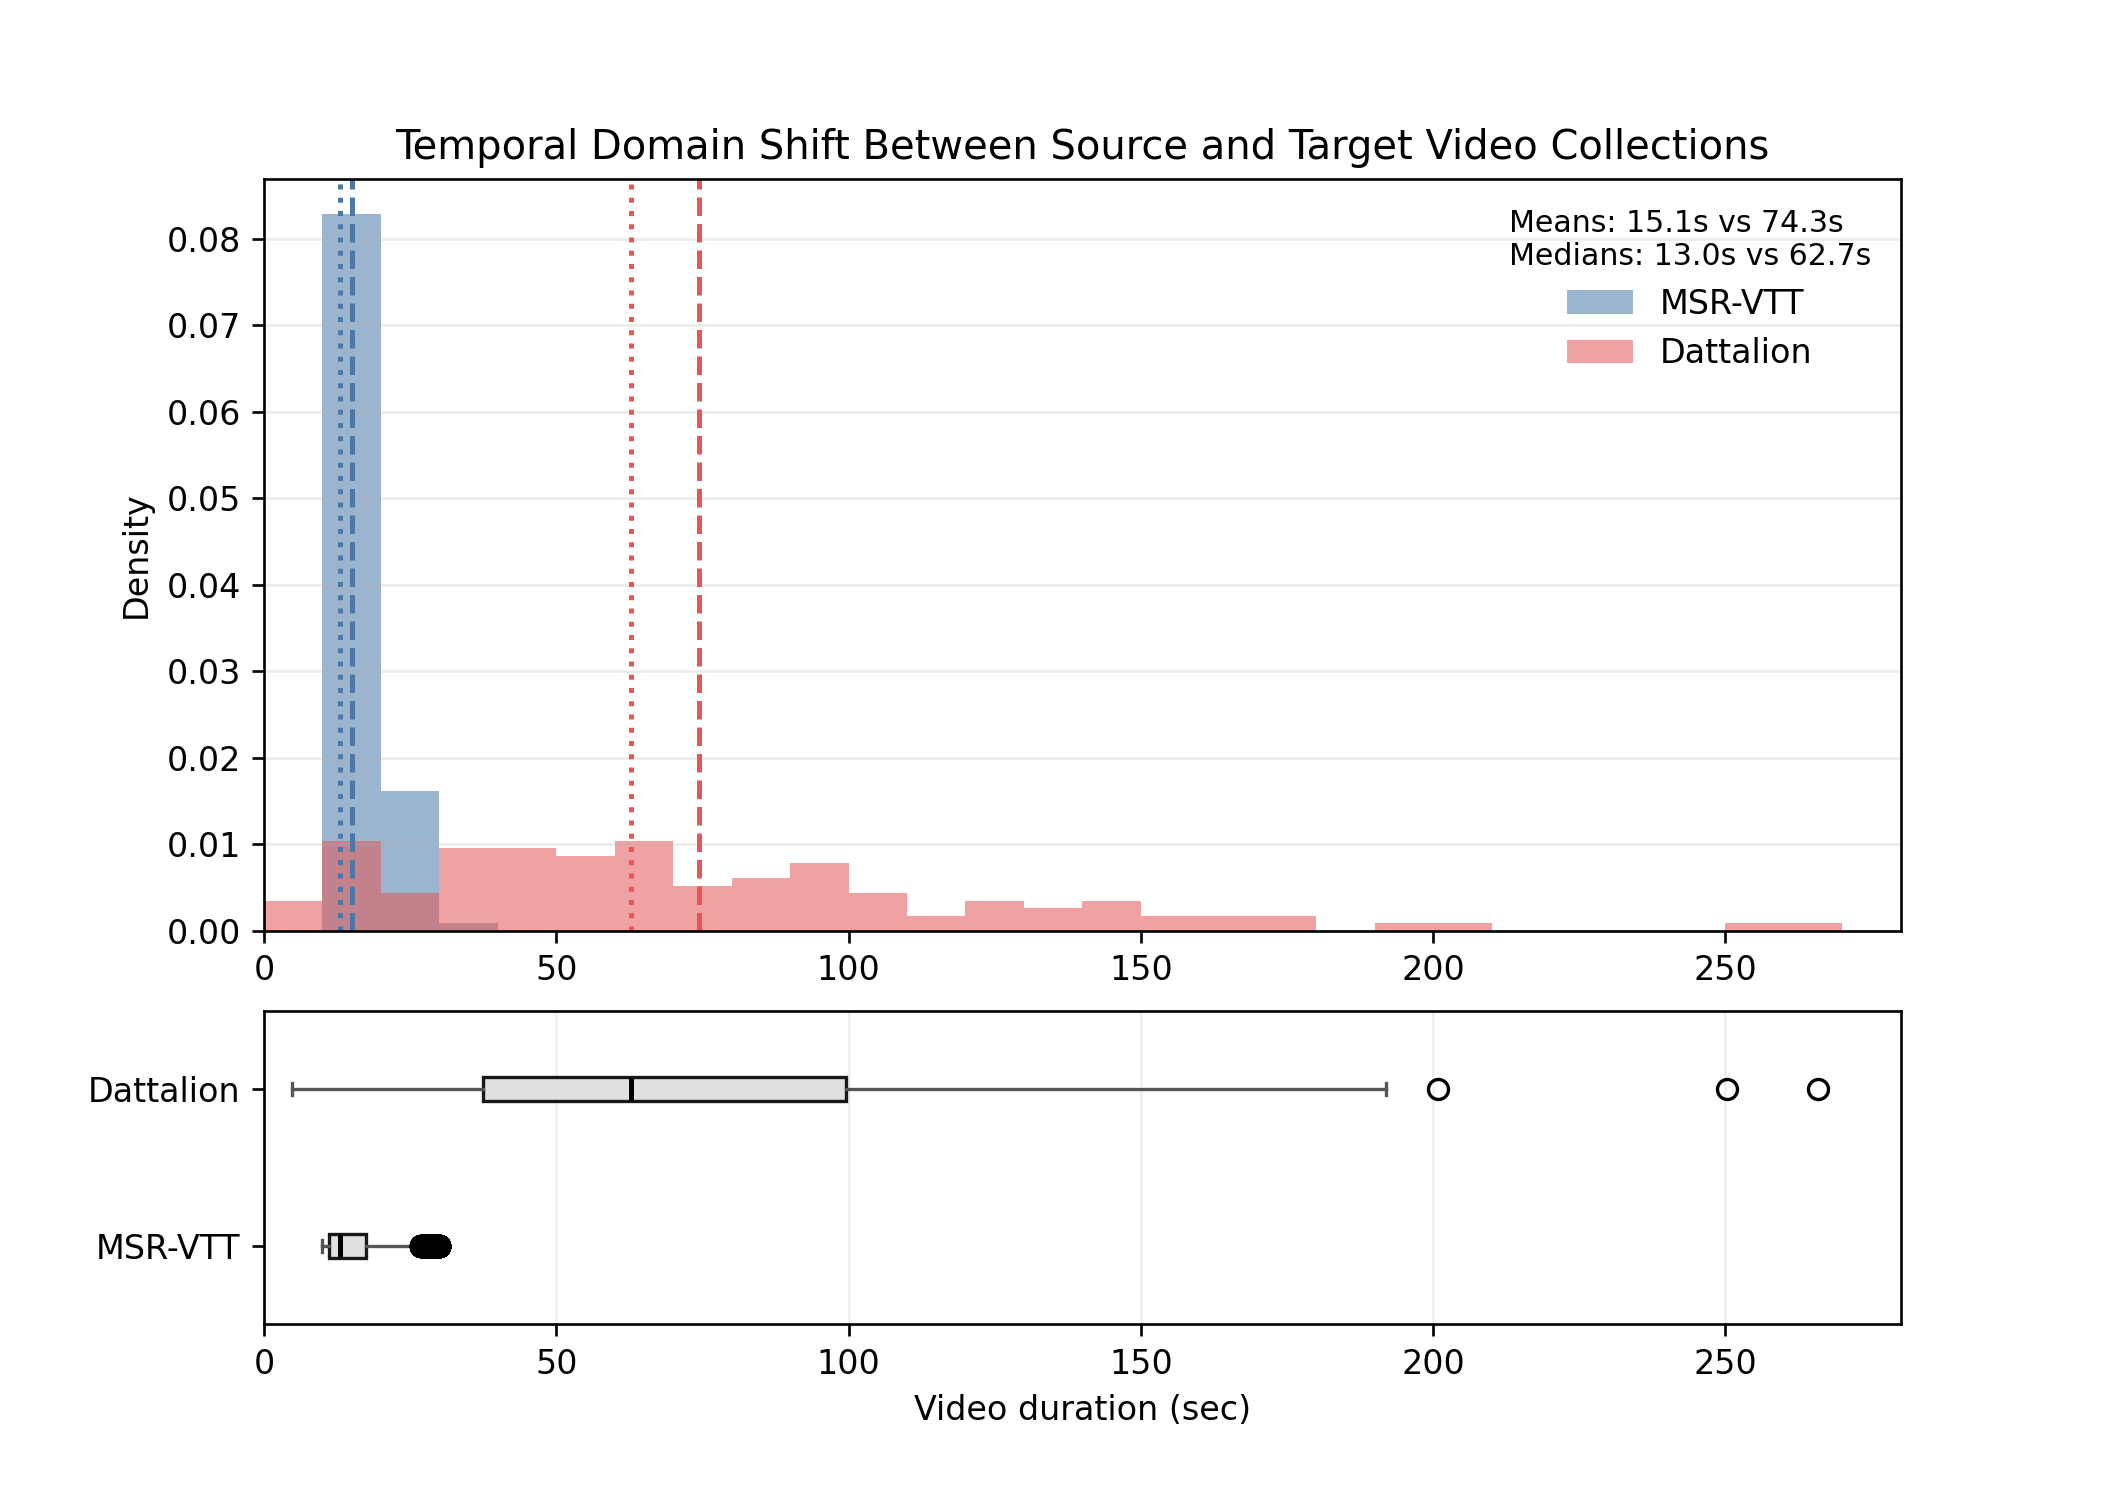
\includegraphics[width=\linewidth]{resubmission_figures/source_target_duration_shift.png}
    \caption{Temporal domain shift between MSR-VTT and Dattalion. The target-domain videos are substantially longer and more variable in duration.}
    \label{fig:duration_shift}
\end{figure}

\subsection{Transfer Protocol}
The transfer protocol has three stages. First, the MSR-VTT model is evaluated on Dattalion without target updates. Second, it is fine-tuned on 0, 10, 20, 30, 40, 50, 60, and 74 target training videos from the fixed 74-video pool and tested on the 30 held-out videos. Because the validation split contains only 10 videos, direct-transfer checkpoints are selected by validation loss rather than volatile validation CIDEr. Third, the final system performs lexical adaptation on curated target captions and applies LV-ECR, a target-side candidate selector whose weights are chosen on the 84 non-test videos and then evaluated once on the held-out test split.

\subsection{Reproducibility and Split Integrity}
The 74 training-pool videos, 10 validation videos, and 30 held-out test videos are mutually disjoint. No Dattalion test videos, test references, normalized test references, or held-out test metrics are used during training, medoid-caption selection, reranker hyperparameter search, or candidate-pool design. Repeated-subset experiments keep the validation and test splits fixed and resample only from the 74-video training pool.

This split discipline is especially important because the target dataset is small enough that accidental leakage would materially change the conclusions. LV-ECR uses the non-test split for feature-weight selection only, and the adaptive BLIP evidence branch is run on held-out videos without using held-out references.

\subsection{Responsible Data Use}
The Dattalion videos are public conflict-related media and may contain damaged infrastructure, emergency response activity, and distressing scenes. They are used only for retrospective captioning research, not for identifying people, inferring operational intent, or geolocating events beyond public source material. Because raw-media redistribution rights may be limited, the reproducibility package focuses on derived artifacts such as split files, captions, manifests, predictions, metrics, and scripts.

\section{Method}\label{sec4}
\subsection{Key-Frame Selection and Visual Representation}
Each video is ultimately represented by a fixed 40-frame visual budget, but the target-domain extractor uses a larger intermediate pool before compression. Candidate frames are sampled at 3 fps for MSR-VTT and 1.5 fps for Dattalion, resized to $224 \times 224$, and encoded with \texttt{openai/clip-vit-base-patch32} and \texttt{facebook/dinov2-base}. Let $f_j$ denote candidate frame $j$, with L2-normalized CLIP and DINOv2 embeddings $c_j$ and $d_j$. The fused embedding used for scoring is
\[
    z_j =
    \frac{[0.55c_j;0.45d_j]}
    {\lVert [0.55c_j;0.45d_j]\rVert_2},
    \qquad
    S_{jk}=z_j^\top z_k ,
\]
where $S_{jk}$ is the cosine similarity between candidates. All scalar cues below are robustly min--max normalized by clipping to the 5th and 95th percentiles before scaling to $[0,1]$.

The local importance score combines six cues:
\[
    I_j =
    0.34s_j + 0.16m_j + 0.06h_j
    + 0.14q_j + 0.14r_j + 0.22p_j .
\]
Here $s_j$ is semantic change, computed from the average distance $1-S_{jk}$ to adjacent candidates; $m_j$ is motion salience from Farneback optical-flow magnitude; $h_j$ is classical color-histogram difference; $q_j$ is image quality from Laplacian sharpness adjusted by exposure; $r_j$ is visual rarity, defined as one minus the mean similarity to the $k=5$ nearest candidates; and $p_j$ is prompt alignment, computed as the maximum CLIP text-image similarity between $f_j$ and the prompt bank. The prompt term is what makes the extractor transfer-aware: it gives additional weight to frames aligned with generic captioning prompts and Dattalion-relevant concepts such as damaged structures, smoke, fire, emergency response, and wide scene context.

For Dattalion, the extractor first chooses an adaptive raw budget before returning to the fixed 40-frame decoder budget. Let $K=40$ be the final budget, $T$ the video duration, $T_{\mathrm{ref}}=14.78$ seconds the MSR-VTT mean duration, and $\delta$ the density of semantic boundary scores above the 92nd percentile. The raw budget is
\[
    K_{\mathrm{raw}} =
    \min\left(
        K_{\max}, M,
        \max\left(K, K_{\min},
        \operatorname{round}\left(K\sqrt{\frac{T}{T_{\mathrm{ref}}}}
        \left(1+0.75\delta\right)\right)\right)
    \right),
\]
where $M$ is the number of sampled candidates, $K_{\min}=40$, and $K_{\max}$ is the raw-pool cap. The reported Dattalion ablations use $K_{\max}=80$ and $K_{\max}=120$. Thus longer videos and videos with more semantic boundaries receive denser candidate coverage, while the downstream captioner still sees exactly 40 frames.

Raw selection is coverage-aware rather than purely top-$I_j$. Semantic scene boundaries are detected from local peaks in adjacent-frame embedding distance, with a 2-second minimum scene length and a 20-second maximum scene length. The greedy selection step first seeds high-scoring scenes, then repeatedly selects the candidate with maximum gain
\[
    G_j =
    I_j + 0.55\Delta C_j + 0.15\mathbb{1}\{\mathrm{newScene}(j)\}
    -0.30R_j ,
\]
where $\Delta C_j$ is the additional similarity coverage obtained by adding $j$, $\mathbb{1}\{\mathrm{newScene}(j)\}$ rewards scenes not yet represented, and $R_j$ is the maximum similarity between $j$ and any already selected frame. This term discourages near-duplicate frames while preserving coverage across the long target video.

If $K_{\mathrm{raw}}>40$, the raw set is compressed back to the final captioning budget in a scene-aware pass. Each represented scene $\ell$ receives a quota based on
\[
    A_\ell =
    0.50\overline{I}_\ell
    + 0.20D_\ell
    + 0.30\overline{p}_\ell ,
\]
where $\overline{I}_\ell$ is mean local importance, $D_\ell$ is normalized scene duration, and $\overline{p}_\ell$ is mean prompt alignment. Within each scene, candidate frames are ranked by
\[
    B_j =
    0.60I_j + 0.25\mathrm{cent}_j + 0.15b_j ,
\]
where $\mathrm{cent}_j$ is similarity centrality within the scene and $b_j$ is the normalized boundary strength. The selected frames are then sorted chronologically. For each final frame, the 512-dimensional CLIP embedding and 768-dimensional DINOv2 embedding are concatenated into a $(40,1280)$ visual tensor and cached before caption-model training.

\subsection{Audio Representation}
Audio is encoded with a VGGish-style 128-dimensional embedding stack \cite{DBLP_VGGish}. Mono 16 kHz waveforms are converted to 64-bin log-mel features with a 25 ms window and 10 ms hop, grouped into 96-frame windows, and passed through VGGish. The resulting variable-length audio token sequences are projected into the shared 512-dimensional multimodal space, masked to ignore padding, and appended to the visual tokens.

\subsection{Caption Decoder}
The decoder is based on \texttt{facebook/bart-base} \cite{lewis2020bart}. The external multimodal encoder projects CLIP and DINOv2 features into a 512-dimensional space, applies CLIP self-attention, cross-attends CLIP queries to DINOv2 keys and values, projects the fused sequence to BART's 768-dimensional hidden size, and passes it directly to the BART decoder as encoder states. BART's text encoder is bypassed.

On MSR-VTT, freezing BART is more stable and yields better performance than fully trainable BART. The final source model therefore freezes BART and trains only the external fusion and projection layers, leaving approximately 3.22M of 142.64M parameters trainable. Generation uses beam search. The Dattalion lexical-adaptation run reported below uses 5 epochs, batch size 2, learning rate $10^{-5}$, and beam-4 and beam-8 candidate pools; the executable scripts record the remaining run configuration, random seeds, and artifact paths.

\subsection{Target-Domain Lexical Adaptation and LV-ECR Reranking}
Direct Dattalion fine-tuning produces useful candidates but unstable top-1 decoding, so the final system separates lexical adaptation from candidate selection. The visual backbone is kept fixed, and only a limited BART lexical subset remains trainable: token embeddings, decoder position embeddings, decoder embedding-layer normalization, decoder output layer normalization, and the tied language-model head. The strongest adapted run initializes from the best frozen direct-transfer checkpoint, trains for 5 epochs with batch size 2 and learning rate $10^{-5}$, and uses each video's five medoid captions as separate training instances.

This lexical-adaptation setting leaves approximately 42.61M of 142.64M parameters trainable and does not update the external multimodal encoder. The use of medoid captions is intended to reduce supervision noise without introducing test-set information.

Beam-4 and beam-8 candidates from this adapted model are then reranked with long-video evidence-calibrated reranking (LV-ECR). The candidate order used for all clean comparisons is recomputed from generation model scores; stored candidate files are not assumed to be in model-score order. LV-ECR adds an evidence branch by captioning eight adaptive key frames per video with BLIP \cite{li2022blip}. The BLIP captions are not emitted as final predictions. Instead, they provide video-level evidence terms for damage, debris, fire, smoke, buildings, people, roads, and emergency response.

For each BART candidate, LV-ECR scores model-relative likelihood, model-rank penalty, visual-evidence alignment, repeated evidence support across key frames, target lexical score, domain-term count, length penalty, repetition penalty, and a small list of generic failure patterns. The weights are selected by grid search on the 84 non-test videos with constraints that require positive visual-alignment and evidence-support weights. The selected setting uses weights of 2.0 for model-relative score, 0.05 for rank penalty, 0.5 for visual alignment, 0.25 for evidence support, 0.2 for target lexical score, 0.05 for length penalty, 0.2 for repetition penalty, and 1.0 for generic failure penalties, with zero domain-count bonus and no switching margin. The candidate-pool oracle reported below selects, for each test video, the highest-CIDEr caption already present in that video's beam set; it is a diagnostic ceiling rather than a deployable system. Figure~\ref{fig:architecture} summarizes the full source-training, target-adaptation, and reranking pipeline.

\begin{figure}[htbp]
    \centering
    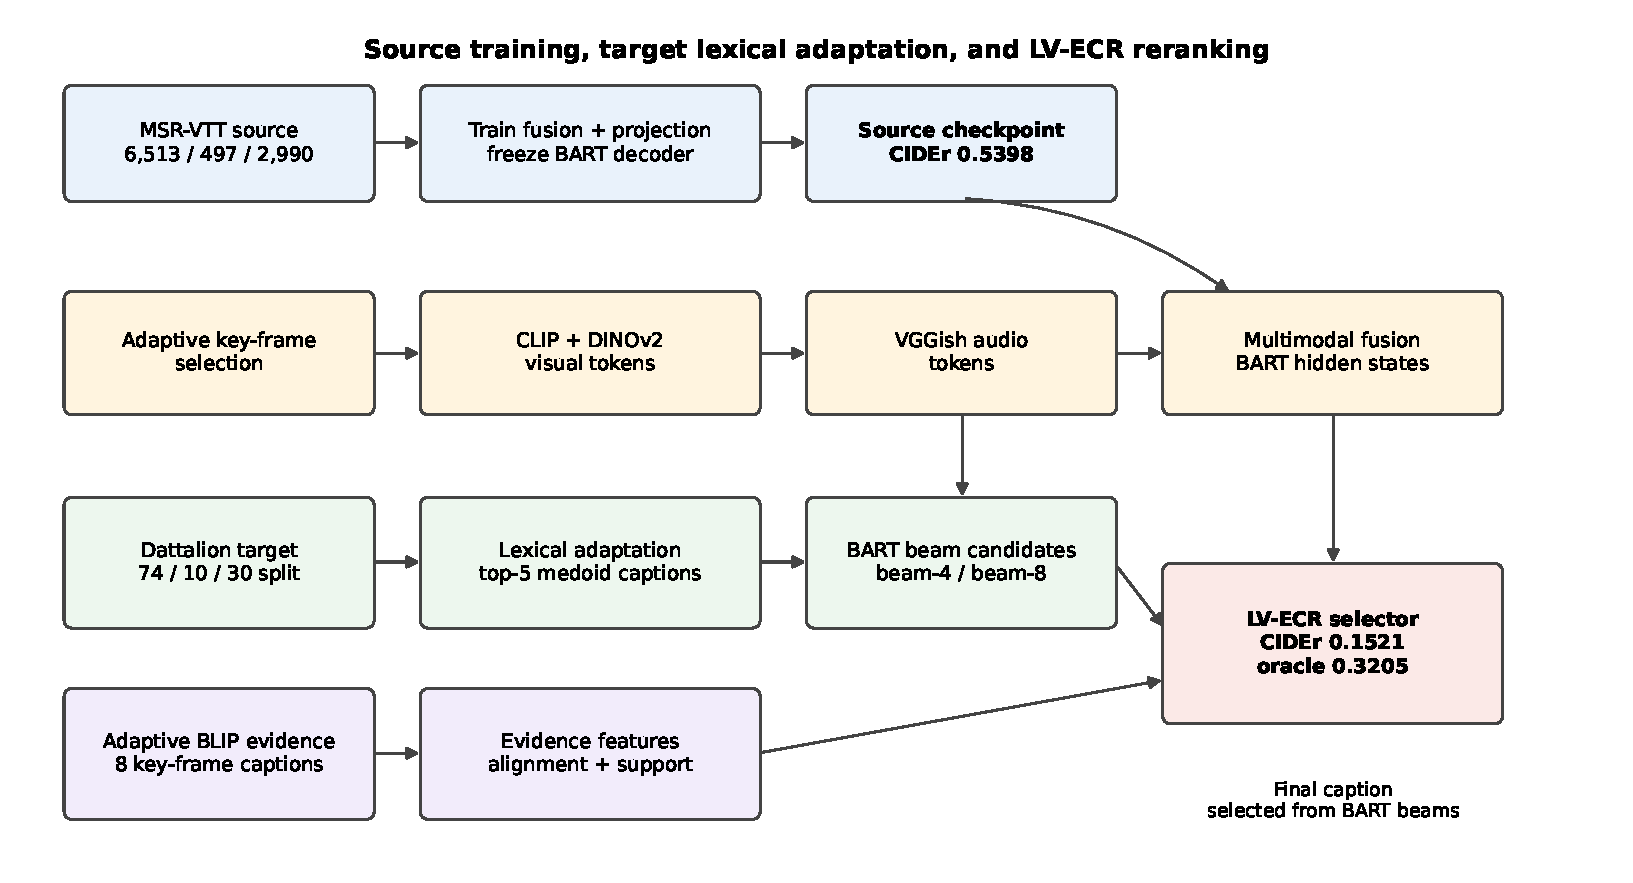
\includegraphics[width=\linewidth]{resubmission_figures/network_architecture.pdf}
    \caption{Multimodal captioning and transfer pipeline. Selected key frames are encoded with CLIP and DINOv2, audio is encoded with VGGish, fused tokens are projected into BART hidden space, and target-domain adaptation performs lexical tuning followed by beam-candidate reranking.}
    \label{fig:architecture}
\end{figure}

\section{Source-Domain Experiments}\label{sec5}
\subsection{Ablation-Based Model Selection}
Figure~\ref{fig:ablation_summary} summarizes the source-domain ablations. Three patterns matter for the transfer study. First, DINOv2 adds substantial value beyond CLIP alone. Second, audio provides an additional gain on top of the two visual streams. Third, freezing the BART decoder outperforms fully trainable BART on the full MSR-VTT split.

\begin{figure}[htbp]
    \centering
    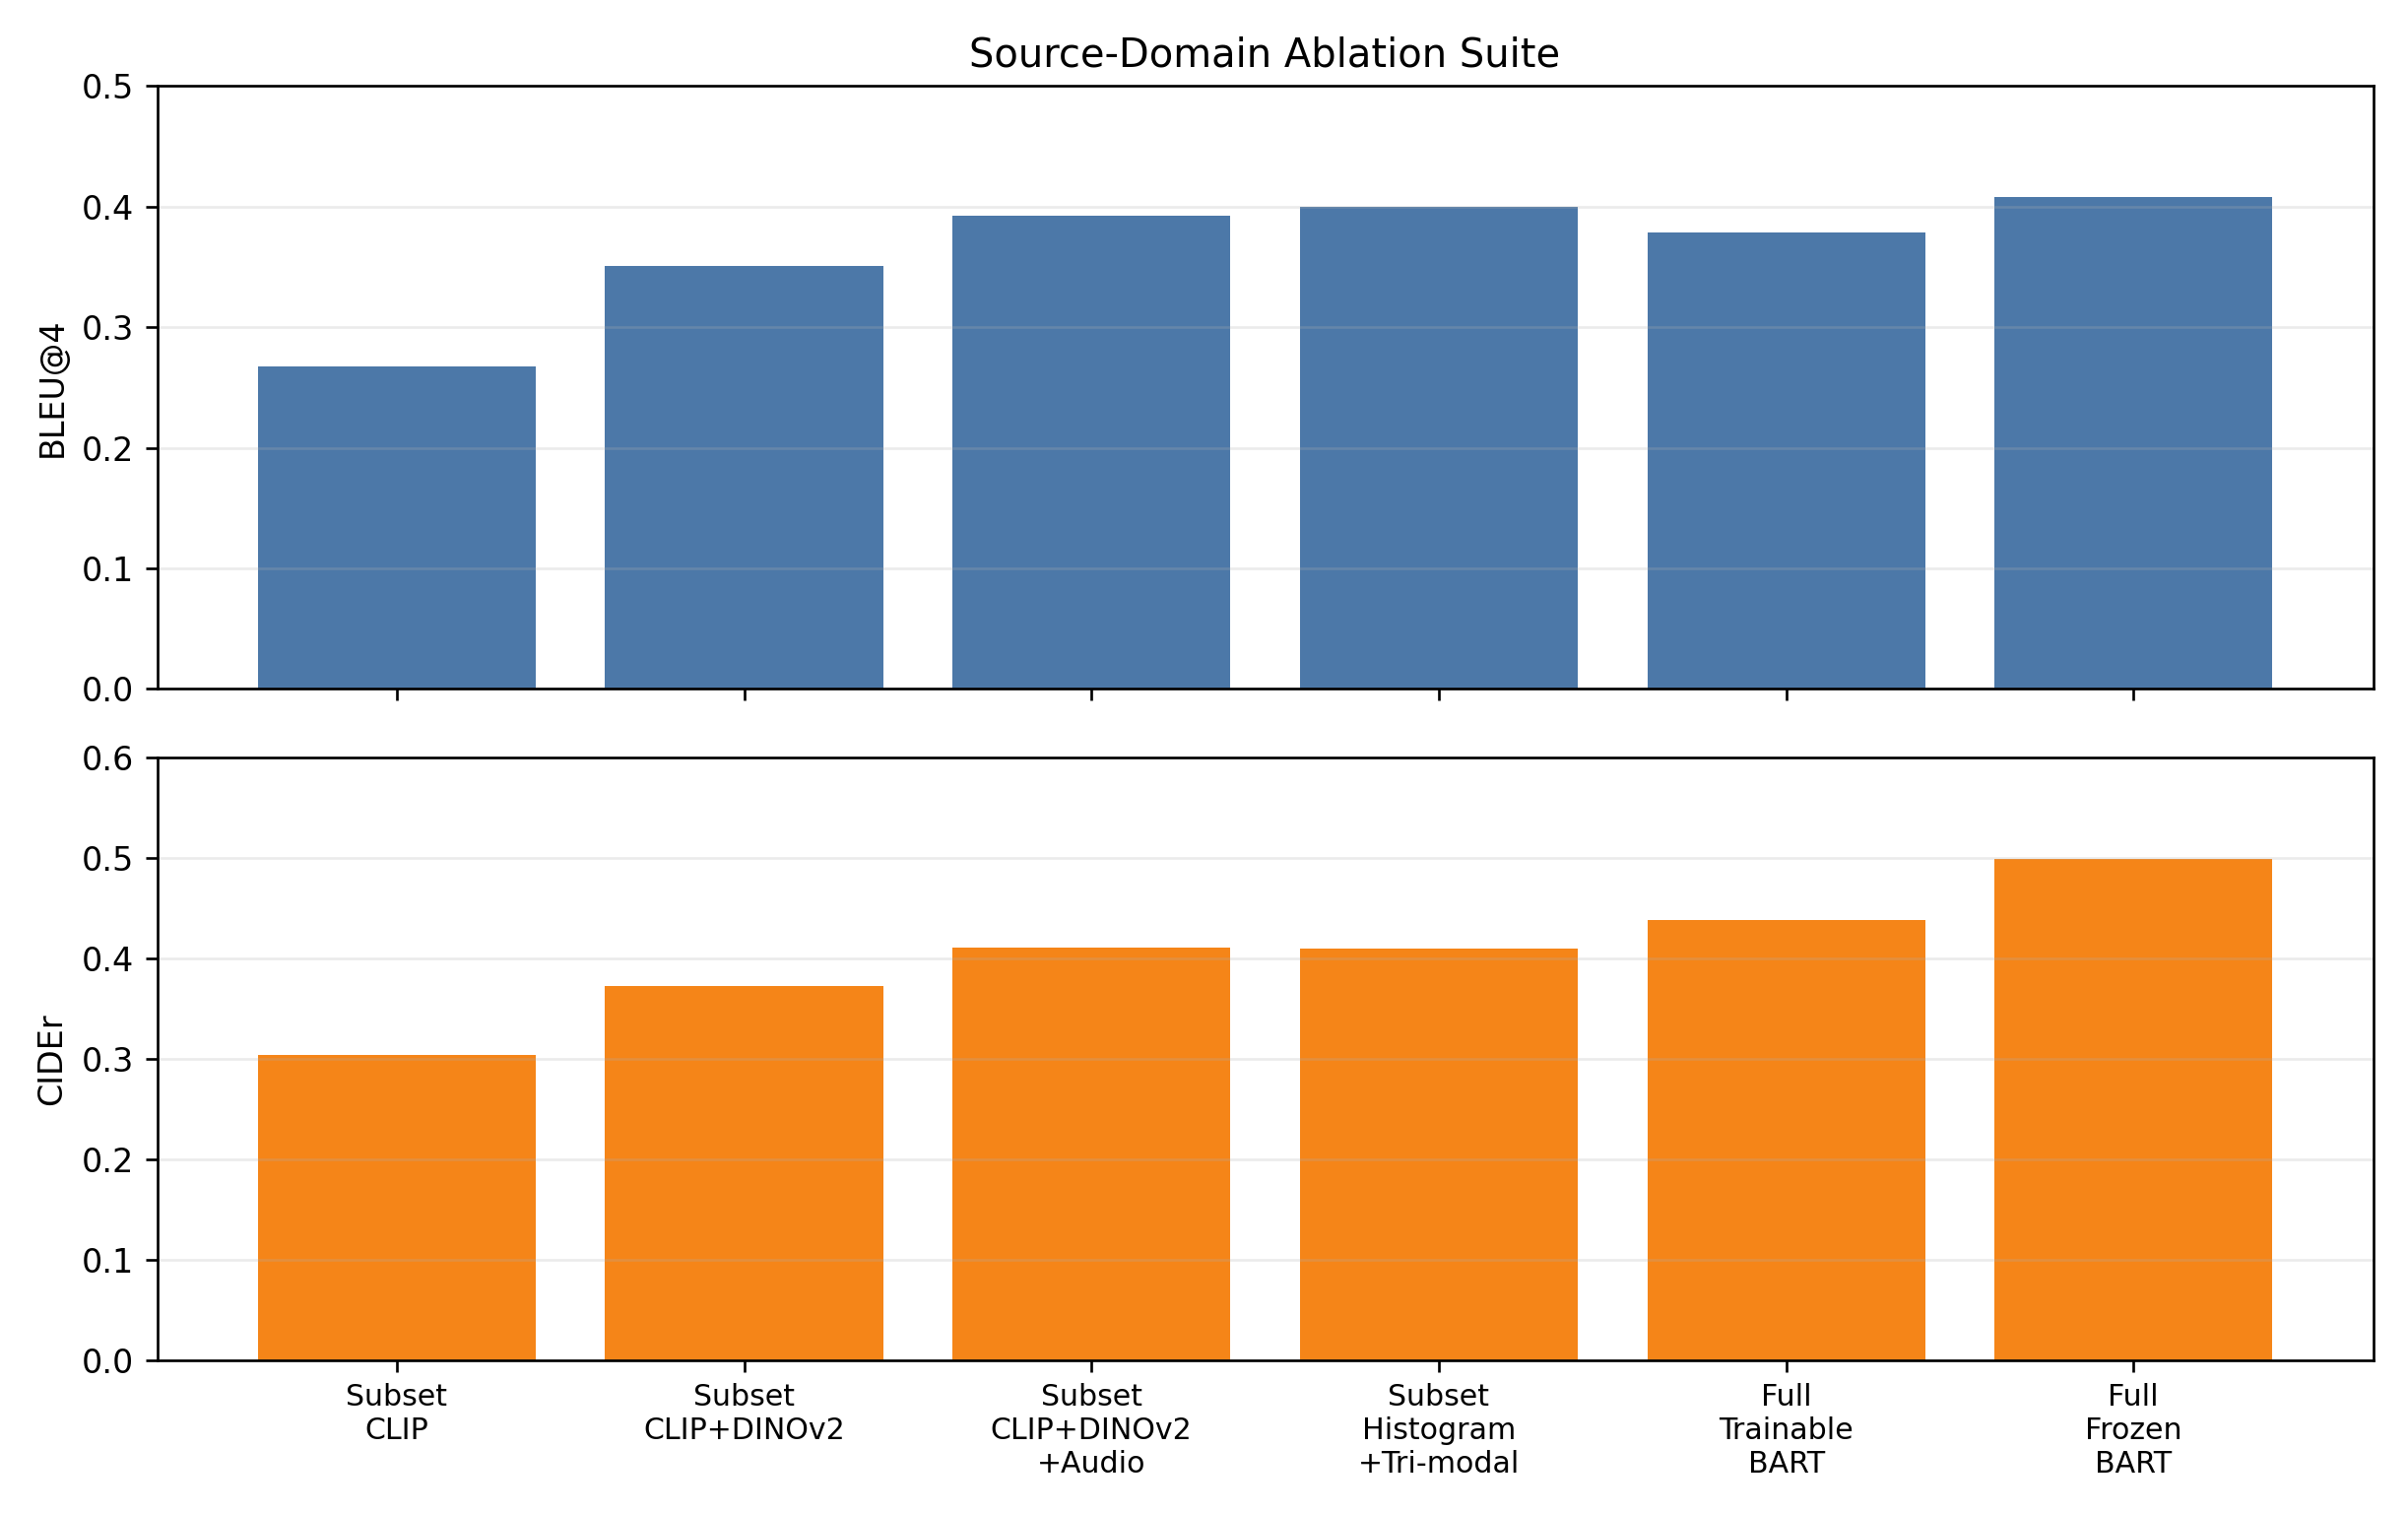
\includegraphics[width=\linewidth]{resubmission_figures/ablation_summary.png}
    \caption{Source-domain ablation summary. The strongest configuration combines CLIP, DINOv2, and audio with a frozen BART decoder.}
    \label{fig:ablation_summary}
\end{figure}

The tri-modal frozen-BART model reaches 0.4081 BLEU@4 and 0.4995 CIDEr on full MSR-VTT. A continuation-style refinement of that same architecture produces the final source-domain model used for transfer, reaching 0.4348 BLEU@4 and 0.5398 CIDEr on the MSR-VTT test set.

These source-domain results establish a reasonably strong starting point for transfer. The purpose of the Dattalion experiments is therefore not to diagnose a weak source model, but to test whether a source model that performs well on a standard short-video benchmark remains useful when temporal length, domain vocabulary, and reference consistency all shift at once.

\begin{table}[htbp]
    \centering
    \begin{tabular}{lcccc}
        \toprule
        \textbf{Source-domain model} & \textbf{BLEU@4} & \textbf{METEOR} & \textbf{ROUGE-L} & \textbf{CIDEr} \\
        \midrule
        Trainable BART & 0.3782 & 0.5365 & 0.5738 & 0.4384 \\
        Frozen BART & 0.4081 & 0.5629 & 0.5977 & 0.4995 \\
        Tuned frozen BART & 0.4348 & 0.5704 & 0.6104 & 0.5398 \\
        \bottomrule
    \end{tabular}
    \caption{Source-domain model selection on full MSR-VTT. The tuned frozen-BART system is used as the source model for transfer.}
    \label{tab:source_models}
\end{table}

\section{Target-Domain Transfer Results}\label{sec6}
\subsection{Direct Few-Shot Transfer Curve}
Figure~\ref{fig:modern_transfer_curve} shows the primary direct-transfer curve on the original Dattalion references. Zero-shot transfer reaches only 0.0491 CIDEr. Direct target adaptation improves quickly at 10 and 20 labeled videos, then becomes non-monotonic as larger fixed subsets do not consistently improve held-out performance. The dashed lines show the clean adapted model-score baseline, LV-ECR, and the diagnostic oracle of the same candidate pool.

We report standard captioning and machine-translation metrics, including BLEU, METEOR, ROUGE-L, and CIDEr \cite{papineni2001bleu,banerjee2005meteor,lin2004rouge,vedantam2015cider}, but emphasize CIDEr, METEOR, ROUGE-L, and lower-order BLEU because the Dattalion references are short and lexically diverse; four-gram BLEU is brittle in this setting.

The direct curve is important because it separates two effects that are easy to conflate. Target supervision clearly helps: 10 labeled videos raise CIDEr to 0.0921, and 20 labeled videos raise it to 0.1031. However, the fixed-subset curve alone does not justify a simple ``more target videos always solve transfer'' conclusion, because the 30-video checkpoint falls to 0.0804 and later checkpoints depend on the adaptive long-video feature setting.

The strongest direct-transfer row in Table~\ref{tab:transfer_anchor_points} uses the 74-video adaptive120 configuration. This is not simply a larger target-training condition; it also reflects the long-video frame-coverage change introduced in Section~\ref{sec4}. The comparison therefore supports two narrower claims: target labels are necessary, and target videos benefit from denser pre-compression coverage before the fixed decoder budget is applied. LV-ECR adds a smaller but positive gain by using adaptive visual evidence to select among candidates already produced by the adapted decoder.

\begin{figure}[htbp]
    \centering
    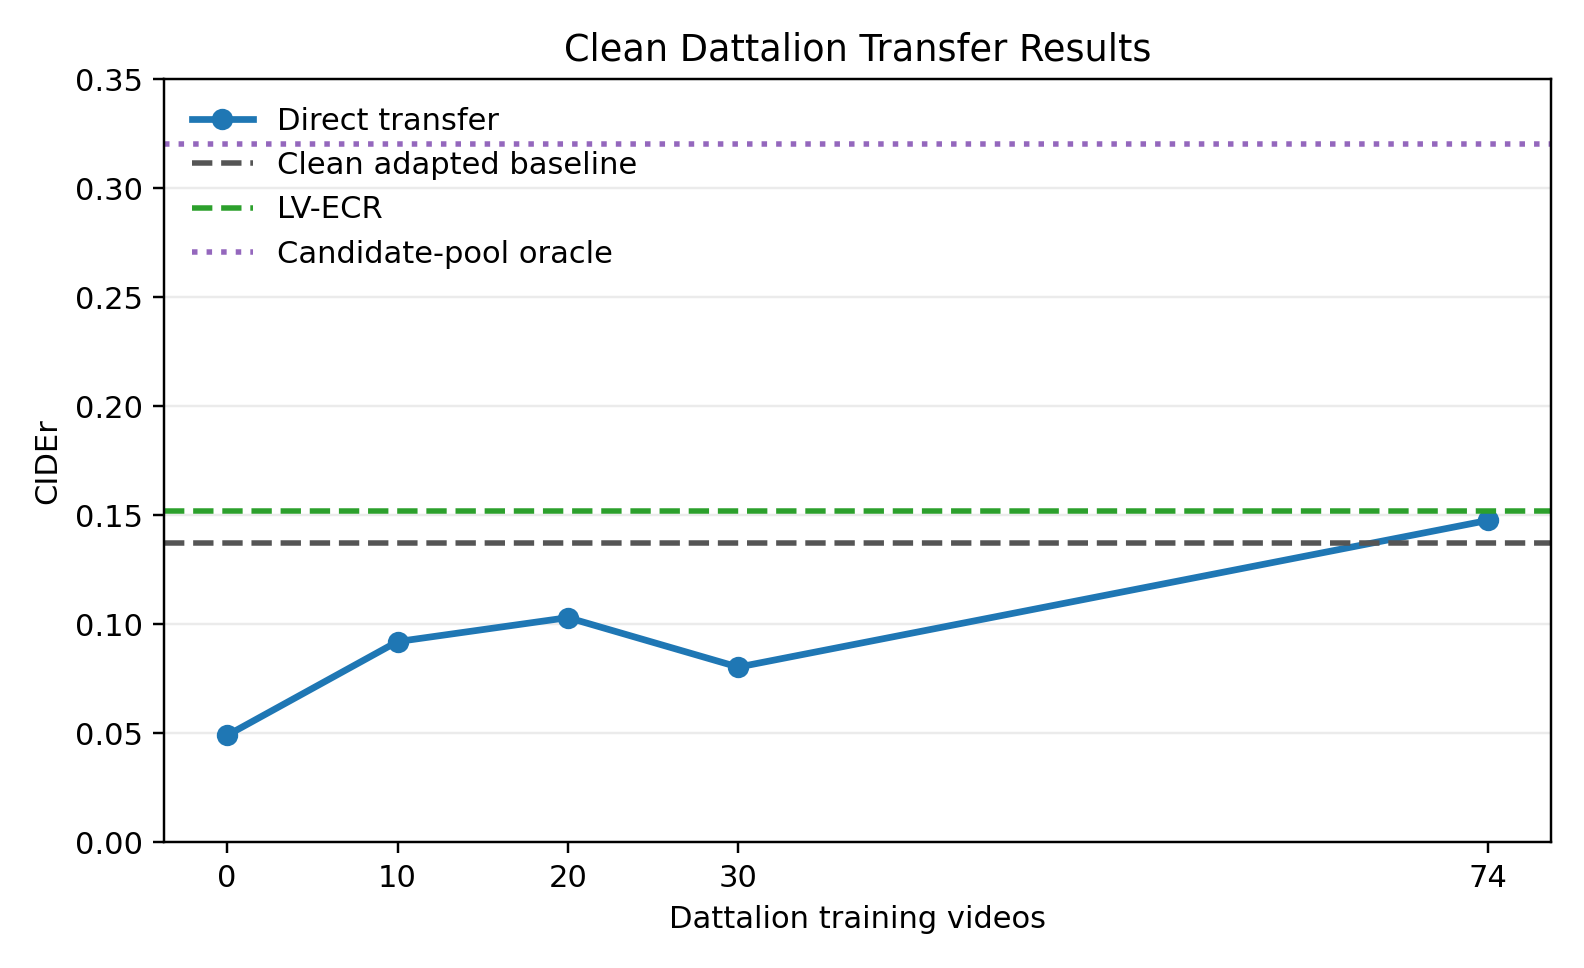
\includegraphics[width=\linewidth]{resubmission_figures/dattalion_transfer_curve_clean_lvecr.png}
    \caption{Direct few-shot transfer curve on Dattalion using the selected source-domain model. Direct target fine-tuning helps quickly, but gains saturate and become non-monotonic as the target training size increases. Dashed horizontal lines show the clean adapted model-score baseline, LV-ECR, and the oracle score of the same candidate pool.}
    \label{fig:modern_transfer_curve}
\end{figure}

\begin{table}[htbp]
    \centering
    \resizebox{\linewidth}{!}{%
    \begin{tabular}{lccccc}
        \toprule
        \textbf{Setting} & \textbf{BLEU@1} & \textbf{BLEU@2} & \textbf{METEOR} & \textbf{ROUGE-L} & \textbf{CIDEr} \\
        \midrule
        0-shot source only & 0.3702 & 0.1472 & 0.1367 & 0.2009 & 0.0491 \\
        10-shot direct & 0.4389 & 0.1857 & 0.1975 & 0.2710 & 0.0921 \\
        20-shot direct & 0.4591 & 0.2027 & 0.1926 & 0.2652 & 0.1031 \\
        30-shot direct & 0.4640 & 0.2141 & 0.1786 & 0.2689 & 0.0804 \\
        74-shot adaptive120 direct & 0.6224 & 0.3624 & 0.2790 & 0.3336 & 0.1477 \\
        \midrule
        Clean adapted model-score baseline & 0.5962 & 0.3324 & 0.2744 & 0.3232 & 0.1374 \\
        LV-ECR (adaptive visual+support) & 0.6009 & 0.3440 & 0.2885 & 0.3198 & 0.1521 \\
        LV-ECR candidate-pool oracle & 0.7815 & 0.5055 & 0.3776 & 0.4204 & 0.3205 \\
        \bottomrule
    \end{tabular}
    }
    \caption{Representative Dattalion transfer results under the cleaned 74/10/30 executable split. Direct few-shot fine-tuning improves quickly at small target sizes but remains unstable under fixed subset choice. Increasing long-video visual coverage with the adaptive120 configuration produces the strongest direct-transfer checkpoint at 0.1477 CIDEr. LV-ECR reaches 0.1521 CIDEr under clean model-score candidate ordering, while the oracle row shows remaining headroom in the same candidate pool and is not a deployable system.}
    \label{tab:transfer_anchor_points}
\end{table}

\subsection{Repeated Subset Sampling in the Low-Resource Regime}
To separate the fixed-subset curve from subset choice, we repeated direct transfer five times at 10, 20, and 30 target videos, resampling from the fixed 74-video training pool while keeping validation and test splits unchanged. Figure~\ref{fig:repeated_sampling_low_resource} summarizes CIDEr and adds the deterministic 74-video point.

Mean CIDEr rises from $0.0810 \pm 0.0085$ at 10 videos to $0.0912 \pm 0.0217$ at 20 videos and $0.1032 \pm 0.0128$ at 30 videos. Variance is visible, especially at 20 videos, but the low-resource trend is upward rather than random.

This repeated-subset analysis is deliberately limited to the smallest training sizes because that is where target-data scarcity is most acute. It shows that the fixed 30-shot dip should not be read as a universal failure of 30-shot learning; it is partly an artifact of which videos entered that particular subset. The broader conclusion is that few-shot transfer improves on average but remains sensitive to the target examples and validation signal.

\begin{figure}[htbp]
    \centering
    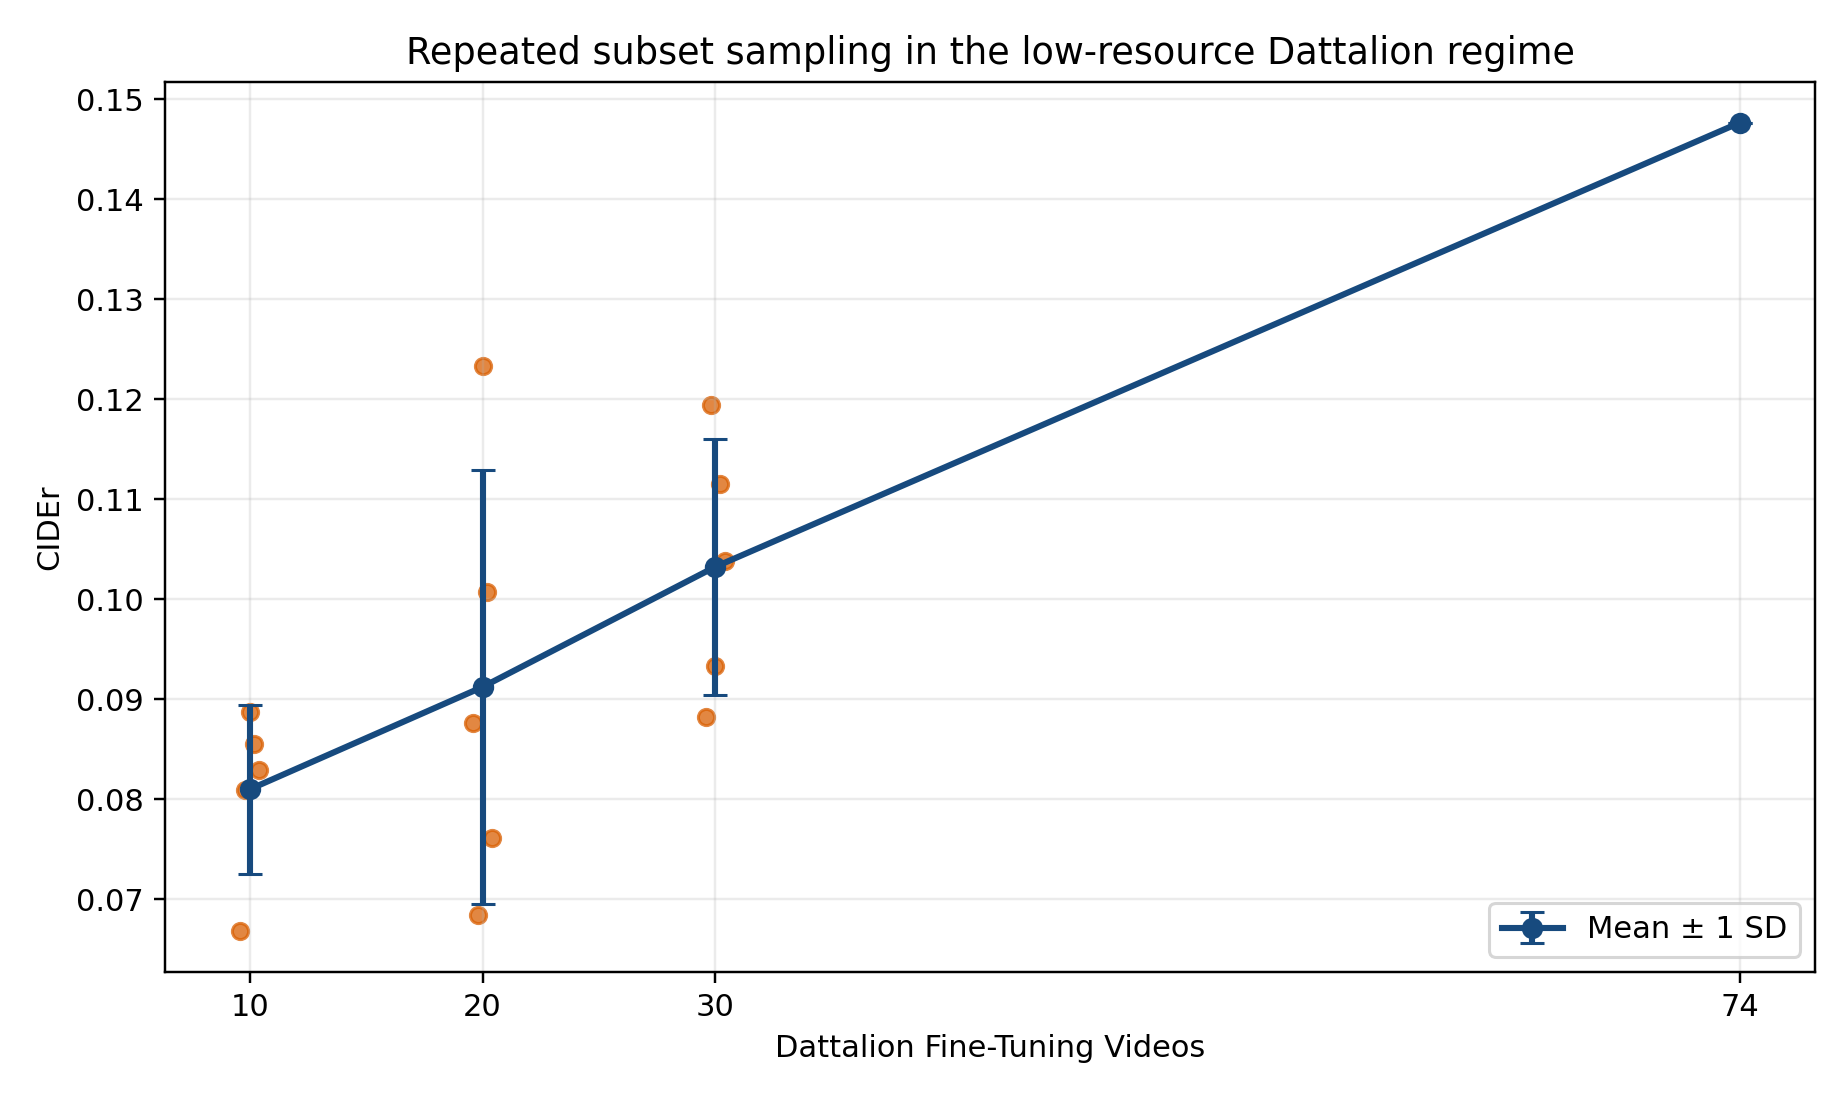
\includegraphics[width=0.95\linewidth]{resubmission_figures/repeated_sampling_cider.png}
    \caption{Repeated subset sampling for direct transfer in the low-resource Dattalion regime. Each point at 10, 20, and 30 training videos is the mean CIDEr over five random draws from the fixed target training pool; error bars show one standard deviation. The 74-video point uses the full target training pool and is therefore deterministic.}
    \label{fig:repeated_sampling_low_resource}
\end{figure}

\subsection{Final Transfer System}
The final system uses the lexical-adaptation-and-LV-ECR stage described in Section~\ref{sec4}. On the 30-video Dattalion test split, the clean adapted model-score baseline reaches 0.1374 CIDEr. LV-ECR raises this to 0.1521 CIDEr and improves METEOR from 0.2744 to 0.2885. The oracle score of the same candidate pool is 0.3205 CIDEr, indicating that candidate generation still leaves substantial headroom for better selection.

The gain should be interpreted conservatively. The paired bootstrap mean sentence-CIDEr improvement over the clean adapted model-score baseline is 0.0145, with a 95\% interval of [-0.0006, 0.0361]. Thus LV-ECR is the strongest clean system in the present experiments, but the uncertainty interval narrowly crosses zero and the evidence is not strong enough to claim a settled statistical advantage.

Figure~\ref{fig:bootstrap_cider} reports bootstrap intervals for the clean adapted model-score baseline and LV-ECR. Both systems select from the same BART candidate pool under model-score ordering; adaptive BLIP captions supply evidence features for LV-ECR but are not used as final captions.

\begin{figure}[htbp]
    \centering
    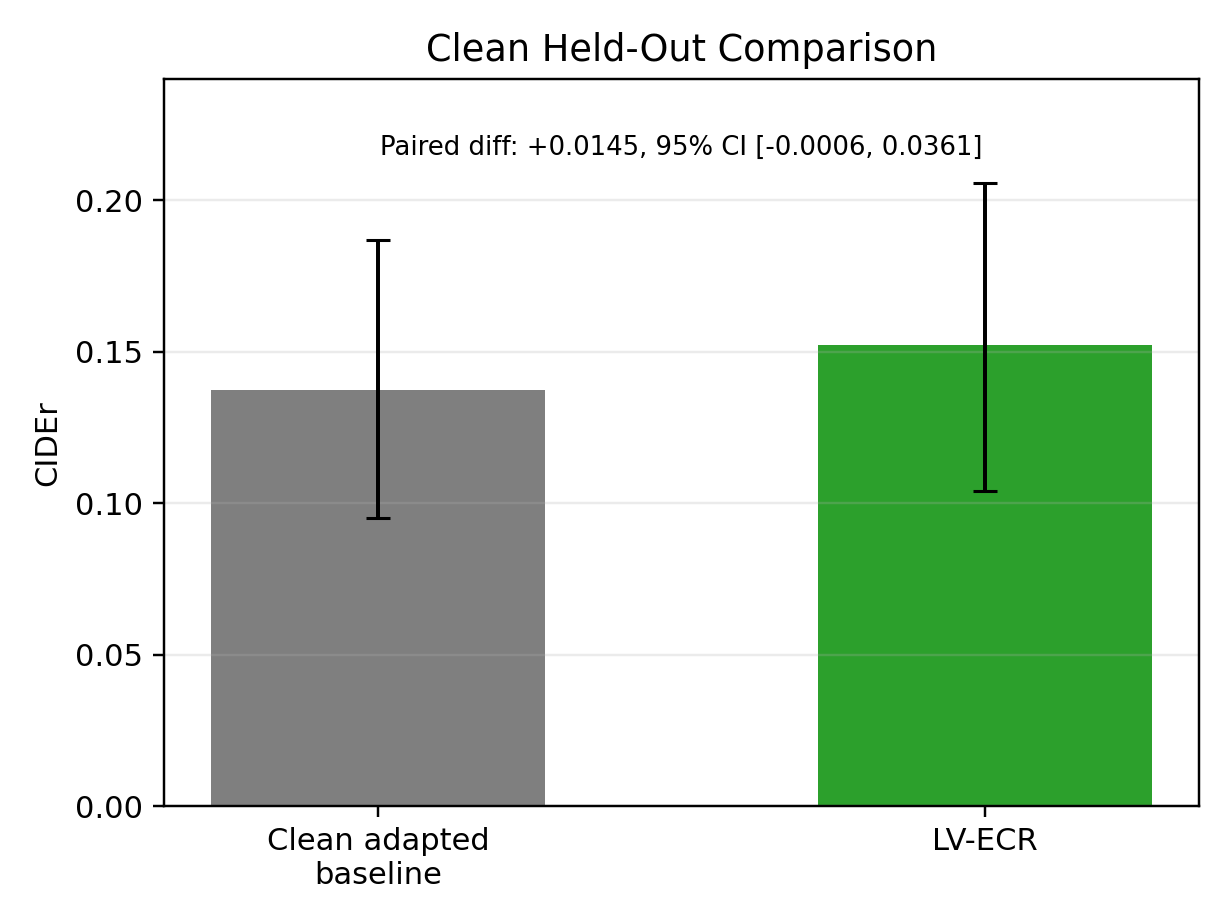
\includegraphics[width=0.95\linewidth]{resubmission_figures/bootstrap_clean_lvecr.png}
    \caption{Mean per-video sentence-CIDEr bootstrap intervals for the clean adapted model-score baseline and LV-ECR on the Dattalion test split. The paired LV-ECR gain is positive on average but the 95\% interval narrowly crosses zero.}
    \label{fig:bootstrap_cider}
\end{figure}

\subsection{Baseline and Reranker Stress Tests}
Table~\ref{tab:baseline_stress} and Figure~\ref{fig:baseline_stress} test retrieval-style transfer, caption-prior transfer, external frame-captioning, and LV-ECR grounding. The nearest-train-video medoid reaches 0.0364 CIDEr, the global target medoid reaches 0.0186, BLIP frame-captioning reaches 0.0827, and GIT reaches 0.0711 under the same three-frame protocol \cite{li2022blip,wang2022git}. These controls support the interpretation that the final result is not explained by a generic conflict-domain caption prior or simple framewise captioning.

The external BLIP and GIT systems are included as sanity checks rather than exhaustive competing long-video systems: each captions three evenly spaced frames independently and then reduces the three captions to a medoid. Even under this modest role, they are useful because they show that a strong image-caption prior applied framewise is not enough to match the adapted video-conditioned system. LV-ECR also improves over the clean adapted model-score baseline while selecting only from the adapted BART beam pool, which keeps the final system tied to video-conditioned candidate generation rather than free-form text post-processing.

LV-ECR variant ablations are reported in Table~\ref{tab:lvecr_variants}. The unconstrained grid gives only a small gain over the clean baseline. Requiring positive visual-evidence weight improves CIDEr, and the strongest clean variant combines visual alignment with repeated key-frame support. These ablations limit the claim: the evidence branch helps, but the improvement is modest and depends on the adapted decoder having plausible candidates in its beam pool.

\begin{table*}[htbp]
    \centering
    \small
    \resizebox{\textwidth}{!}{%
    \begin{tabular}{lccccccccc}
        \toprule
        \textbf{Method} & \textbf{Vid.} & \textbf{Caps.} & \textbf{Ext.} & \textbf{BLEU@2} & \textbf{METEOR} & \textbf{ROUGE-L} & \textbf{CIDEr} & \textbf{Key cov.} \\
        \midrule
        Caption prior medoid & -- & $\checkmark$ & -- & 0.1143 & 0.1741 & 0.1775 & 0.0186 & 100.0\% \\
        Train-neighbor retrieval & $\checkmark$ & $\checkmark$ & $\checkmark$ & 0.1267 & 0.2021 & 0.2109 & 0.0364 & 90.0\% \\
        BLIP frame-caption baseline & $\checkmark$ & -- & $\checkmark$ & 0.1729 & 0.2085 & 0.2361 & 0.0827 & 53.3\% \\
        GIT frame-caption baseline & $\checkmark$ & -- & $\checkmark$ & 0.1790 & 0.1949 & 0.2378 & 0.0711 & 43.3\% \\
        Source-only transfer & $\checkmark$ & -- & $\checkmark$ & 0.1472 & 0.1367 & 0.2009 & 0.0489 & 16.7\% \\
        Strongest direct transfer & $\checkmark$ & $\checkmark$ & $\checkmark$ & 0.3624 & 0.2790 & 0.3336 & 0.1477 & 83.3\% \\
        Clean adapted model-score baseline & $\checkmark$ & $\checkmark$ & $\checkmark$ & 0.3324 & 0.2744 & 0.3232 & 0.1374 & 90.0\% \\
        LV-ECR & $\checkmark$ & $\checkmark$ & $\checkmark$ & 0.3440 & 0.2885 & 0.3198 & 0.1521 & 93.3\% \\
        \bottomrule
    \end{tabular}
    }
    \caption{Baseline and reranker stress tests on the Dattalion test set. ``Vid.'' indicates whether the method uses the test video itself, ``Caps.'' whether it uses target-domain training captions, and ``Ext.'' whether it relies on external pretraining. ``Key cov.'' is the fraction of test captions containing at least one non-test Dattalion keyword. Caption-prior and retrieval controls remain below the adapted video-conditioned systems, and framewise BLIP/GIT baselines do not match LV-ECR.}
    \label{tab:baseline_stress}
\end{table*}

\begin{table}[htbp]
    \centering
    \small
    \begin{tabular}{lccc}
        \toprule
        \textbf{Variant} & \textbf{METEOR} & \textbf{ROUGE-L} & \textbf{CIDEr} \\
        \midrule
        Clean model-score baseline & 0.2744 & 0.3232 & 0.1374 \\
        LV-ECR, unconstrained grid & 0.2725 & 0.3090 & 0.1397 \\
        LV-ECR, visual-positive & 0.2741 & 0.3122 & 0.1443 \\
        LV-ECR, visual+support+margin & 0.2622 & 0.3109 & 0.1467 \\
        LV-ECR, visual+support & 0.2885 & 0.3198 & 0.1521 \\
        \bottomrule
    \end{tabular}
    \caption{Clean LV-ECR variant ablations on the Dattalion test set. The strongest variant requires both visual alignment and repeated key-frame evidence support, but the gain over the clean model-score baseline remains modest.}
    \label{tab:lvecr_variants}
\end{table}

\begin{figure}[htbp]
    \centering
    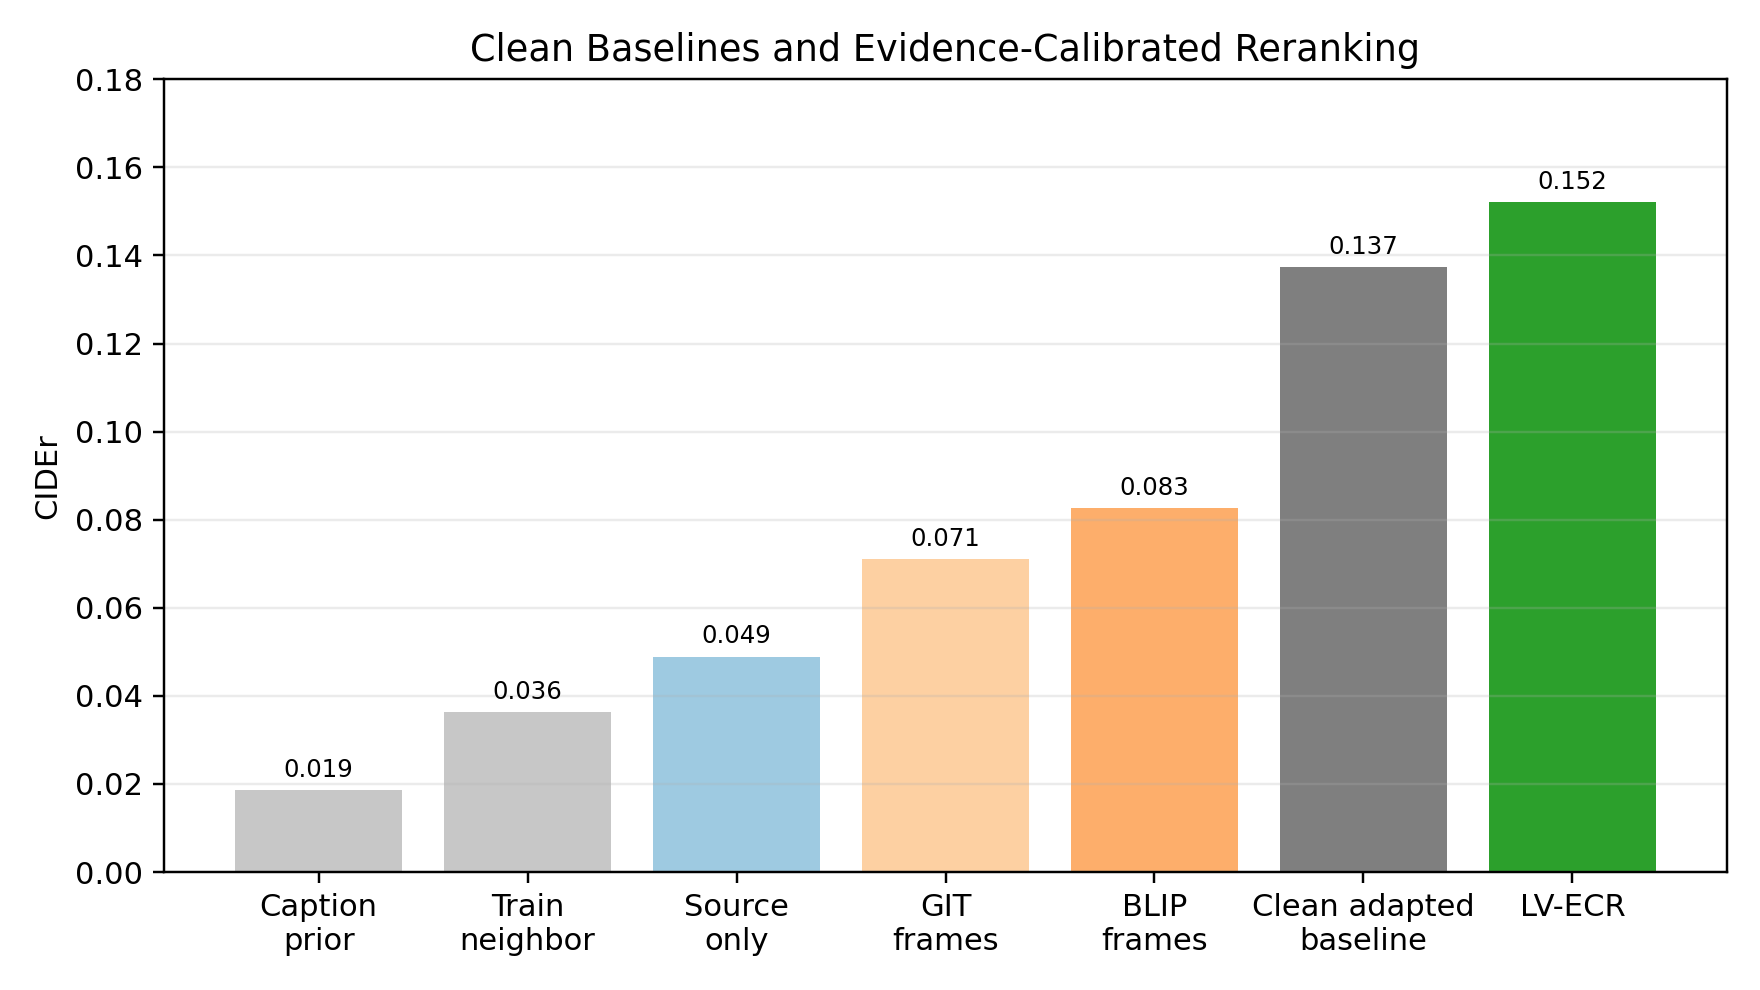
\includegraphics[width=\linewidth]{resubmission_figures/clean_baseline_stress_lvecr.png}
    \caption{Stress tests for the final transfer system. The left panel shows CIDEr for key baselines and grounding controls; the right panel shows keyword coverage. High keyword coverage by itself is not sufficient, as shown by the caption-prior control.}
    \label{fig:baseline_stress}
\end{figure}

\subsection{Target-Domain Transfer Ablations}
Figure~\ref{fig:dattalion_transfer_ablations} summarizes the clean Dattalion-side ablations. Increasing the adaptive raw pool from 80 to 120 frames raises direct-transfer CIDEr from 0.1212 to 0.1477. Lexical adaptation with clean model-score ordering reaches 0.1374 CIDEr. LV-ECR then improves the adapted candidate selector to 0.1521 CIDEr, with the visual+support variant performing best among the clean reranking settings.

\begin{figure}[htbp]
    \centering
    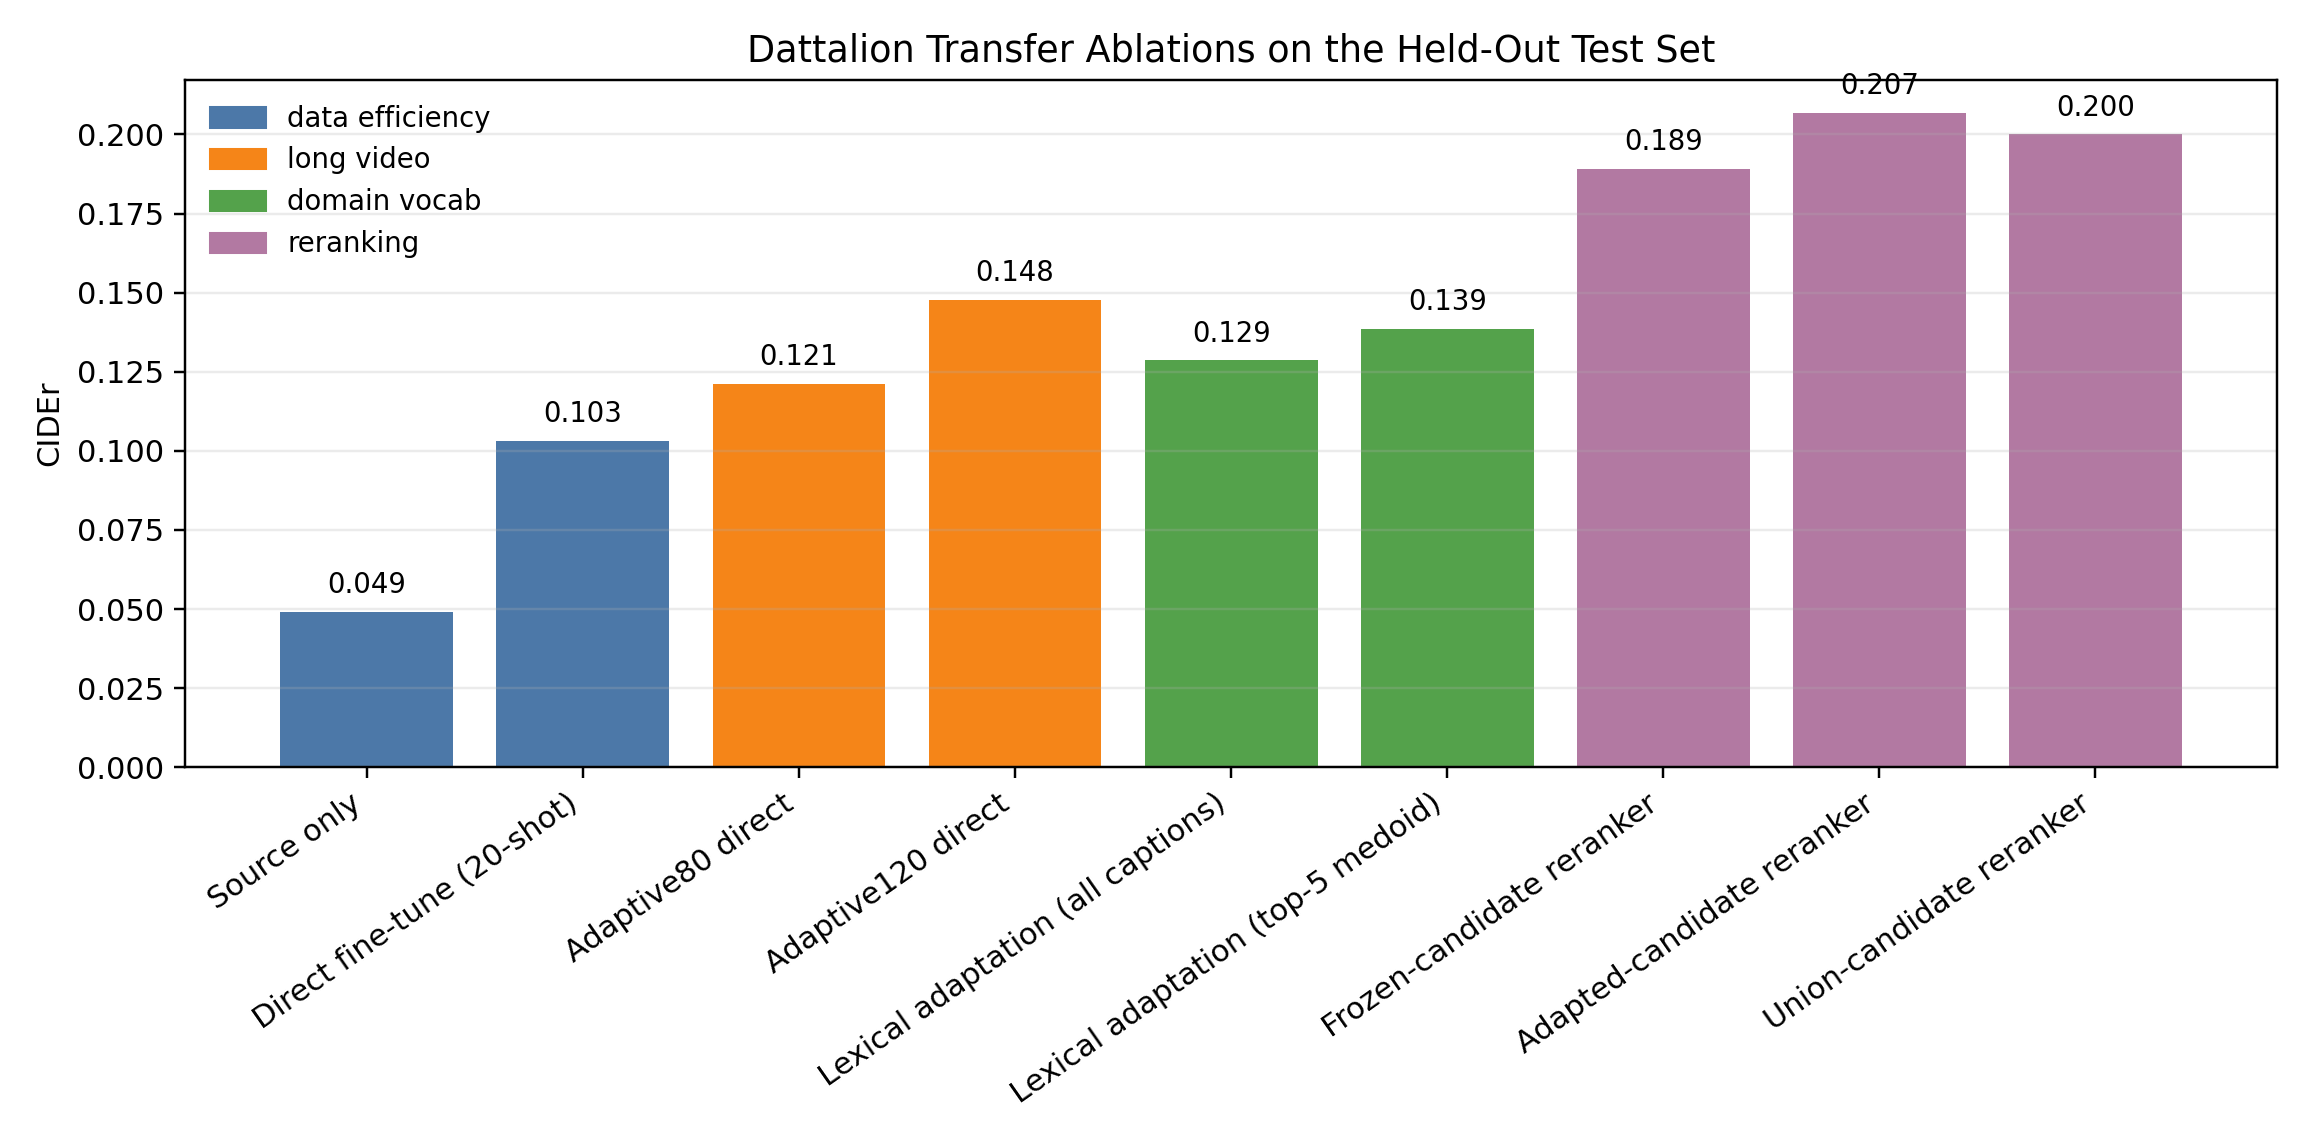
\includegraphics[width=\linewidth]{resubmission_figures/dattalion_transfer_ablation_cider.png}
    \caption{Clean Dattalion test-set ablations for transfer learning. Adaptive long-video features provide the strongest direct-transfer gain; LV-ECR adds a smaller gain by using adaptive visual evidence to select among clean model-score-ordered candidates.}
    \label{fig:dattalion_transfer_ablations}
\end{figure}

\subsection{Domain-Specific Vocabulary Transfer}
To probe lexical grounding, we build a keyword bank from non-test Dattalion captions using high-frequency words such as \textit{building}, \textit{fire}, \textit{damaged}, \textit{debris}, \textit{firefighters}, and \textit{rubble}. As shown in Figure~\ref{fig:keyword_coverage}, the zero-shot source model uses a domain keyword in only 16.7\% of Dattalion test captions. The strongest direct adaptive120 model reaches 83.3\%, the clean adapted baseline reaches 90.0\%, and LV-ECR reaches 93.3\%.

This keyword analysis is intentionally simple. It is not treated as a semantic correctness metric, since a caption can contain a domain word and still describe the wrong event. Its value is diagnostic: the source-only system rarely enters the target vocabulary at all, whereas target adaptation changes the lexical content of the predictions even when exact n-gram scores remain modest.

\begin{figure}[htbp]
    \centering
    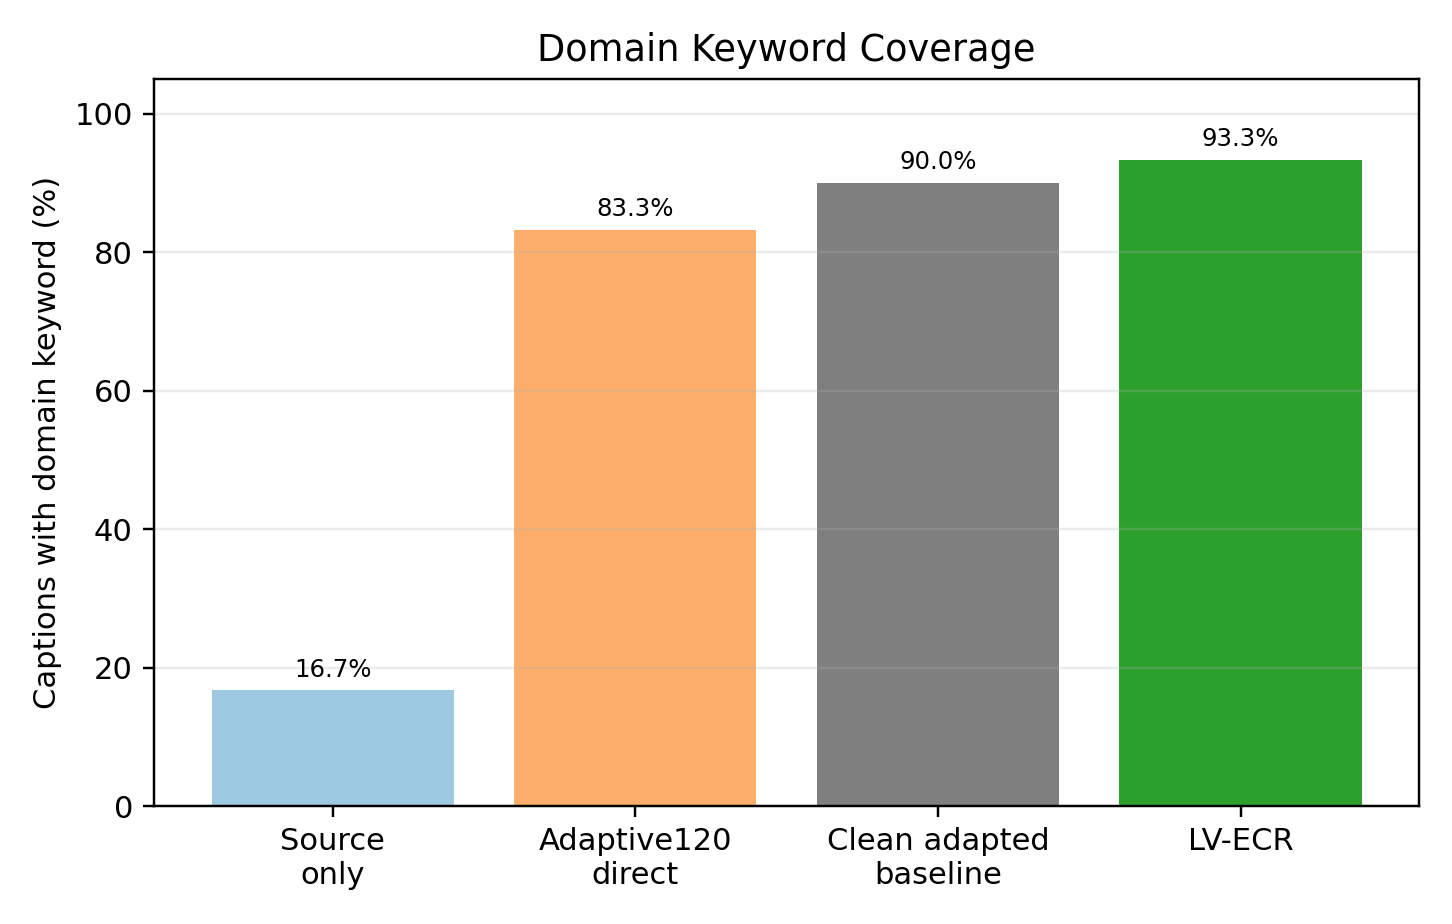
\includegraphics[width=0.95\linewidth]{resubmission_figures/domain_keyword_coverage_clean_lvecr.png}
    \caption{Domain-specific keyword coverage on the Dattalion test set. Few-shot target adaptation sharply increases the fraction of captions that mention domain-relevant concepts, while LV-ECR adds a small further increase.}
    \label{fig:keyword_coverage}
\end{figure}

\subsection{Reference Consistency and Transfer Stability}
\label{sec:reference_agreement}
The Dattalion references are much less lexically aligned than MSR-VTT references. Average pairwise token-level Jaccard agreement is 0.059 for Dattalion and 0.162 for MSR-VTT, a 2.7$\times$ reduction (Figure~\ref{fig:reference_agreement}). This makes exact n-gram metrics conservative because valid target descriptions may use different surface forms.

The original Dattalion references remain the primary evaluation. As a sensitivity test, we also construct a conservative normalized-caption variant that preserves scene content while reducing wrapper phrases and uncontrolled synonym drift. The rules are defined before rescoring, do not use model outputs, and are applied only when the original caption set supports the normalized wording.

Under normalized references, Dattalion agreement rises from 0.0590 to 0.1285. Matched 20-shot adaptive120 reruns show that consistency also affects learning: original captions yield 0.0980 and 0.0902 CIDEr under validation-loss and validation-CIDEr checkpointing, while normalized captions yield 0.1387 and 0.2120 under the same selection rules. Separately, direct-transfer rescoring under normalized references raises the strongest direct model from 0.1487 to 0.2262 CIDEr. We do not use normalized captions to select or report the clean LV-ECR result; they are a sensitivity analysis showing that target-caption consistency affects evaluation and checkpointing.

The normalization rules remove wrappers such as \textit{footage of} and \textit{scene shows}, harmonize recurring nouns such as \textit{debris}, \textit{rubble}, and \textit{damaged building}, and standardize actor labels within a video only when the original caption set already supports a dominant choice. Thus captions such as ``footage of cracked walls and broken stonework'' and ``wide shot of ruined stone building'' can be mapped toward a shared event focus without rewriting the underlying scene. This keeps the original references as the main benchmark while showing how much lexical variability suppresses both evaluation and validation-based model selection.

The matched reruns in Table~\ref{tab:normalized_20shot_deconfound} are included for this reason. They do not claim that normalized captions should replace the original benchmark, and they do not rerun the full final system. Instead, they isolate a training-stability effect: when train, validation, and test captions use more consistent wording, the same small validation split becomes more informative for checkpoint selection. That effect is directly relevant to low-resource transfer, where a 10-video validation set can otherwise reward the wrong checkpoint.

\begin{table}[htbp]
    \centering
    \small
    \begin{tabular}{llc}
        \toprule
        \textbf{Caption protocol} & \textbf{Checkpoint selection} & \textbf{CIDEr} \\
        \midrule
        Original captions & Validation loss & 0.0980 \\
        Original captions & Validation CIDEr & 0.0902 \\
        Normalized captions & Validation loss & 0.1387 \\
        Normalized captions & Validation CIDEr & 0.2120 \\
        \bottomrule
    \end{tabular}
    \caption{Matched 20-shot adaptive120 direct-transfer reruns under the current target-transfer recipe. The only changes are the target caption protocol and the checkpoint-selection criterion.}
    \label{tab:normalized_20shot_deconfound}
\end{table}

\begin{figure}[htbp]
    \centering
    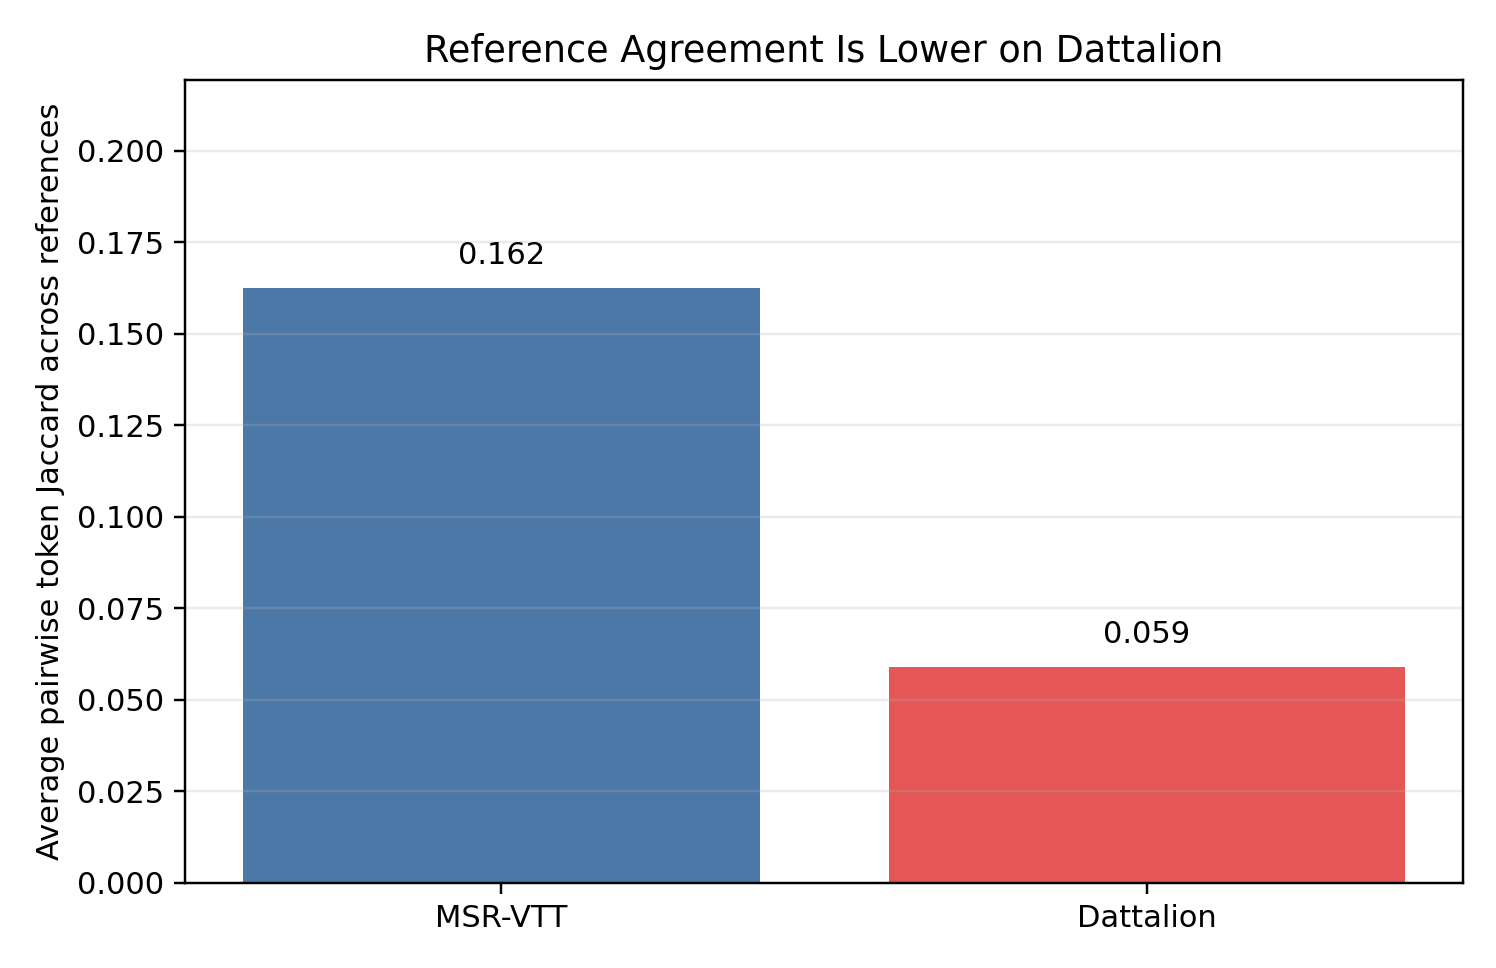
\includegraphics[width=0.92\linewidth]{resubmission_figures/reference_agreement.png}
    \caption{Average pairwise token-level Jaccard agreement among references. Dattalion references are much less lexically aligned than MSR-VTT references, which helps explain why low-resource transfer is sensitive to caption normalization and checkpoint selection.}
    \label{fig:reference_agreement}
\end{figure}

\subsection{Qualitative Behavior}
The qualitative examples follow the keyword analysis. Source-only captions are often generic, while adapted captions become more domain-specific but can still miss the event. Table~\ref{tab:dattalion_cases} includes a clear improvement, a partial improvement, and a failure case for LV-ECR relative to the clean adapted baseline.

\begin{table*}[htbp]
    \centering
    \small
    \setlength{\tabcolsep}{3pt}
    \begin{tabular}{@{}>{\raggedright\arraybackslash}p{0.16\linewidth}>{\raggedright\arraybackslash}p{0.19\linewidth}>{\raggedright\arraybackslash}p{0.18\linewidth}>{\raggedright\arraybackslash}p{0.18\linewidth}>{\raggedright\arraybackslash}p{0.18\linewidth}@{}}
        \toprule
        \textbf{Case} & \textbf{Representative reference} & \textbf{Source-only caption} & \textbf{Clean adapted caption} & \textbf{LV-ECR caption} \\
        \midrule
        Clear improvement\\(\texttt{video10021}) & people looking at rubble and destroyed road & a man talks about his car & scene shows broken pavement and debris & damaged road shows broken pavement and debris \\
        Partial improvement\\(\texttt{video10006}) & firefighters work to put out fire & a truck drives through a field & firefighters use hose to clear debris & firefighters use fire hose to clear debris \\
        Failure / repetition\\(\texttt{video10028}) & multiple firetrucks fight fire at large building & a fire breaks out & firefighters and firefighters work on the roof of a large building & firefighters and firefighters work on the roof of a building under heavy fire \\
        \bottomrule
    \end{tabular}
    \caption{Representative Dattalion transfer examples. The first row shows a clear gain in domain grounding, the second a partial gain with residual event mismatch, and the third a failure case where LV-ECR remains in-domain lexically but retains repetition and incomplete event grounding.}
    \label{tab:dattalion_cases}
\end{table*}

\section{Discussion}\label{sec7}
The results show that strong source-domain captioning does not automatically yield strong transfer. The selected model is effective on MSR-VTT, but zero-shot Dattalion performance is poor because the target domain differs in temporal structure, vocabulary, and reference consistency. The target set is not merely a smaller or harder version of MSR-VTT; it asks the model to compress longer videos and produce captions in a narrower operational vocabulary.

Target supervision helps quickly but remains unstable under direct fine-tuning. Repeated subset sampling improves on average from 10 to 30 videos, and the strongest direct checkpoint uses adaptive long-video coverage. However, direct top-1 decoding still leaves performance on the table: the LV-ECR candidate-pool oracle reaches 0.3205 CIDEr, far above the deployed selector. The keyword analysis supports the interpretation that target adaptation changes the concepts the model mentions, not only its n-gram overlap with references.

A practical implication is that target-domain captioning systems should not be judged only by the size or strength of the source model. In this study, the target-side choices are decisive: how long videos are compressed, which target captions supervise lexical adaptation, how candidates are selected, and whether the validation captions are consistent enough to support checkpointing. These are lower-level experimental details, but in a 74-video training regime they become central modeling decisions.

The normalized-caption reruns show that annotation consistency is part of the transfer problem. The original 10-video validation split is too noisy for CIDEr-based checkpointing, while normalized captions make validation-CIDEr selection much more informative. The effect is therefore not only metric inflation. It changes which checkpoint appears best and shows why a very small, lexically inconsistent target set can make model selection unreliable even when the model is learning domain-relevant language.

The stress tests constrain the reranker claim. Retrieval, caption-prior, BLIP/GIT frame-captioning, bootstrap intervals, and candidate-oracle analysis indicate that the final gain is not just a generic conflict-language prior or simple frame-caption prior. At the same time, the paired bootstrap interval crosses zero, and the final system still selects only among candidates already generated by the adapted decoder. LV-ECR should therefore be read as a transfer-aware candidate-selection improvement, not as a complete solution to long-video event grounding.

The absolute Dattalion scores remain far below the source-domain MSR-VTT score. This is a finding rather than only a weakness of the experiment. It indicates that transfer under simultaneous temporal and semantic shift remains difficult even with a modern multimodal backbone and many references per held-out video. The failure case in Table~\ref{tab:dattalion_cases} illustrates the remaining problem: the model can become lexically in-domain while still missing the actual event.

The main limitations are scale and evaluation breadth. Repeated subset sampling is reported only for the 10-, 20-, and 30-video regime; normalized-caption reruns cover matched 20-shot direct transfer rather than the full 74-shot and LV-ECR stack; and no multi-rater human evaluation is reported for the clean LV-ECR system. These choices keep the added analyses feasible but leave room for stronger evidence. Larger target sets, multi-rater evaluation with agreement measurement, and segment-level long-video modeling would strengthen future work.

\section{Conclusion}\label{sec8}
This paper studies transfer learning for multimodal video captioning under simultaneous temporal and semantic shift. A CLIP, DINOv2, VGGish, and frozen-BART captioner reaches 0.5398 CIDEr on MSR-VTT but only 0.0491 CIDEr when transferred zero-shot to Dattalion, showing that short open-domain benchmark success does not carry over automatically to long conflict-domain videos.

Direct target adaptation helps but is not sufficient. Repeated subset sampling improves from 0.0810 CIDEr at 10 target videos to 0.1032 at 30, and the strongest direct 74-video configuration reaches 0.1477. LV-ECR reaches 0.1521 CIDEr and 93.3\% domain-keyword coverage, compared with 0.1374 CIDEr and 90.0\% keyword coverage for the clean adapted model-score baseline. Bootstrap intervals, stress tests, external frame-caption controls, and candidate-oracle analysis support a conservative conclusion: target-side evidence calibration can help, but the present improvement is modest and should not be overread.

The broader result is that low-resource transfer for long, single-context target videos is a system problem. Strong source models help, but the target side still needs better temporal coverage, curated supervision, reliable candidate selection, and annotation protocols that make small validation sets informative. Future work should prioritize segment-level long-video modeling, visually grounded rerankers, larger target-domain evaluation sets, and multi-rater human evaluation that can capture domain grounding when n-gram metrics remain conservative.

\section*{Funding}
The authors did not receive any funding for this project.

\section*{Author Information}
\subsection*{Authors and Affiliations}
Aidan Looney and Mike Powell conducted this work in the Department of Mathematical Sciences, United States Military Academy, West Point, NY, 10997, United States of America.

\subsection*{Contributions}
All authors contributed to the research design, experiment planning, and manuscript preparation. Data processing, model training, and analysis were performed by Aidan Looney. Mike Powell supervised the project and revised the manuscript. All authors approved the final version.

\subsection*{Corresponding Author}
Mike Powell (mike.powell@westpoint.edu)

\subsection*{Data Availability}
The derived artifacts used for this submission are provided in the accompanying supplementary package, including executable split metadata, prediction files with held-out references, clean LV-ECR configurations and bootstrap summaries, normalized-caption sensitivity summaries, and figure-generation outputs. The package includes a manifest and SHA-256 checksums. Raw Dattalion videos originate from public conflict-media sources with separate platform-level access conditions and are not redistributed in the derived-artifact package.

\section*{Ethical declarations}
\subsection*{Conflict of Interest}
The authors declare no competing interests.

\subsection*{Ethical Approval}
Not applicable. This retrospective study used publicly accessible videos and did not involve intervention with human subjects, collection of personally identifying annotations, or deployment in a live operational setting. Section~\ref{sec3} describes responsible-data restrictions for potentially distressing conflict-related media.

\subsection*{Consent to Participate}
Not applicable.

\subsection*{Consent for Publication}
All authors have read the final version and agreed to submit.

\newpage
\bibliography{sn-bibliography}

\end{document}
